\chapter{Balancing methods}
\label{chap:experiment_3_balancing}

% \textbf{Q4:} What is the effect of using the reproduced methods on the representation of low-resource languages? And
% \textbf{Q5:} How do the reproduced methods compare to the standard method of training the tokenizer on balanced and unbalanced joint corpus?


Finally, we replicate the works of \citet{chung_improving_2020,zheng_allocating_2021,liang_xlm-v_2023} (we colectivelly address these works as the "vocabulary balancing methods") and create several variations of their tokenizers that aim to improve the text segmentations, especially for the low-resource languages. We carefully compare these replicated tokenizers with the traditional method of training Sentencepiece Unigram tokenizers on a joint, multilingual corpus.

By comparing the balancing tokenizers, we aim to answer (\textbf{Q4}) what is the effect of using the balancing methods on the representation of low-resource languages? And (\textbf{Q5}) how do the balancing methods compare to the standard method of training the tokenizer on balanced and unbalanced joint corpus?

Our method is to replicate and train all examined tokenizers and perform the intrinsic and extrinsic evaluation. We will examine closely the overall perfomance, as well as the changes for the individual languages.

The replication of the balancing methods is described in \autoref{sec:reproducing_the_vocabulary_balancing_methods}, then we evaluate closely the tokenizer properties in \autoref{sec:intrinsic_evaluation_of_the_balancing_methods}. Finally, we select a subset of the tokenizers and pretrain masked language models to see the effect of tokenization on the downstream tasks in \autoref{sec:extrinsic_evaluation_of_the_balancing_methods}.


% We then validate our findings by training a second batch of masked language models that differ only in the tokenizer used. We choose the clustering method of \citet{chung_improving_2020} and allocation method of \citet{zheng_allocating_2021} and compare them with Sentencepiece Unigram tokenizers trained on balanced and unbalanced data. 


\section{Reproducing the vocabulary balancing methods}
\label{sec:reproducing_the_vocabulary_balancing_methods}
% - replication of the previous balancing work
%     - the code is not available for Chung and Liang, for Zheng we reimplement even though the code is available
%     - therefore we follow all papers closely
%     - Chung
%         - reproductions of chung are available in the paper Overlap-based Vocabulary Generation Improves Cross-lingual Transfer Among Related Languages
%             - they do not replicate the results of Chung
%         - we run training with 8k vocab size, unigram, coverage 0.9995 (default in Sentencepiece) for each language
%             - this is specified in the paper
%             - we use 1M lines for each language which we have shown to be enough in preliminary experiments
%         - we compute the binary vectors for each language and normalize them to unit length
%         - we compute clusters using k-means, with k=4, 8, 12, 16, 20 (=all languages)
%         - train the tokenizers on the clusters
%             - target vocab size is 120k, again use Sentencepiece defaults
%             - to reach the vocab size we train also +10\%, +20\%, +30\% of the target size and then prune
%         - then we merge the tokenizers

%     - Liang
%         - we follow the same procedure as in Chung
%         - compute negative log-likelihoods for each token over the corpus and use the euclidean distance to compute the similarity
%         - but we use the sizes from Zheng

In this section, we describe our reproduction of the existing methods for balancing the low- and high- resource languages in the vocabulary. As the code for two out of three of the methods is not available, we follow and reimplement the original papers closely and describe the differences in our implementation.

The methods of \citet{chung_improving_2020} and \citet{liang_xlm-v_2023} follow a three step process: 1) grouping the languages into clusters by similarity, 2) running the Unigram LM tokenizer training on the clustered corpora and 3) combining the cluster-vocabularies into a single, multilingual vocabulary. Because of their similarity, we refer to the two as the clustering methods. The method of \citet{zheng_allocating_2021} works in two steps: 1) training the Unigram LM tokenizers for each language separately and 2) selecting the best vocabulary size for each language and combining the vocabularies into a single, multilingual vocabulary.

As we can see the methods share the last merging step and differ in the clustering approaches. We therefore describe the clustering approaches first, then we describe the Zheng method and finally we describe the merging step common for all methods.

\subsection{Reproducing the clustering methods}
% \tomasz{General remark: It's better to keep experiments definition (i.e. hypothesis statement and experiment overview.) separated from implementation details.
% The later are important bu shouldn't steal attention of the reader from the story.}

The first step for the Chung and Liang methods is to train monolingual Unigram LM tokenizers for each language $l$ from the set of 20 languages $L$. As specified in \citet{chung_improving_2020}, we use the default Sentencepiece settings. Namely, we use the Unigram LM model, character coverage of 99.95\%, number of seed sentencepieces is 1M. \xxx{add all parameters to appendix?}. 
For training the monolingual tokenizers, we use 1M lines for each language which we have shown to be enough in preliminary experiments \autoref{sec:data_size}. This choice also corresponds to the \citet{zheng_allocating_2021} method, which uses 1M lines for each language. The vocabulary size differs between Chung and Liang and so we train two sets of monolingual tokenizers, with 8k and 30k vocabulary sizes respectively.

We arrive at $|L|$ vocabularies $V^l$. Next, we take the union of all vocabularies $V^L = \bigcup_{l \in L} V^l$ and compute the "vector representation" $\vec{v}^l$ for each language $l$ as described in \autoref{sec:chung} and \autoref{sec:liang}. For Chung, we compute a binary vector of size $|V^L|$, where each element $\vec{v}^l_i$ is 1 if the token $i$ is in the vocabulary $V^l$ of language $l$ and 0 otherwise. For Liang, we compute a vector of size $|V^L|$, where each element $\vec{v}^l_i$ is the negative log-likelihood of the token $i$ in the language $l$ as computed by the Sentencepiece training algorithm. We set the log-likelihood of the tokens not in the vocabulary to 0 as inferred from the Figure 1 in \cite{liang_xlm-v_2023}. We discuss this choice in more detail in the discussion \autoref{sec:language_vectors}.

With the vector representations $\vec{v}^l$ we can cluster the languages into $k$ clusters $C^k$ using the k-means algorithm. We use the implementation from \texttt{scikit-learn} \cite{pedregosa_scikit-learn_2011} with the default parameters. \citet{chung_improving_2020} reports using the cosine distance for the k-means algorithm. We normalize the language representation vectors to unit length, to achieve the same effect. In the case of Liang, we stick to Euclidean distance as the authors do not mention using a different metric. We experiment with $k \in \{4, 8, 16, 20\}$. Note that $k=20$ corresponds to separating each language into a separate cluster which is similar to the method \textsc{TokMix} we introduce in \citet{limisiewicz_tokenization_2023} and \citet{zheng_allocating_2021} we replicate next.

Then, given a clustering of languages $C$, for each cluster $c_j \in C$ we create a new training corpus by concatenating all of the CC100 data belonging to the cluster\footnote{Because of computational constraints, we cap the total number of lines per cluster to 20M. If the cluster corpus exceeds the total number of lines, we subsample the available data with $\alpha=1.0$}. We run the Sentencepiece algorithm again on these clustered corpora to arrive at cluster-specific vocabularies $V^{c_j}$. The vocabulary size for each cluster is determined following the Chung and Liang methods. For both methods, we want to arrive at the final size of 120k tokens after merging the cluster-specific vocabularies. Therefore we need to determine the size of each cluster vocabulary $|V^{c_j}|$ such that $\sum_{j=1}^k |V^{c_j}| = 120k$. The Chung method sets the size of the cluster vocabulary to be proportional to the size of the union over the monolingual vocabularies $|\bigcup_{l \in c_j} V^l|$ to determine the size of each cluster vocabulary as follows:

\begin{equation}
    |V^{c_j}| = \frac{|\bigcup_{l \in c_j} V^l|}{\sum_{i=1}^k |\bigcup_{l' \in c_i} V^{l'}|} \cdot 120k
\end{equation}

The Liang method proposes to set the size of the cluster vocabulary to be proportional to the sum of the vocabulary allocations from \citet{zheng_allocating_2021} for the languages belonging to the cluster. We use the allocations we reproduce in \autoref{subsec:reproducing_vocap}.
\footnote{
    Here we slightly improve the methods of Chung and Liang. By following the original method as described above, the final size of the vocabulary will be lower than the target we set. This is because the cluster vocabularies $V^{c_j}$ will contain overlapping tokens and merging will remove these duplicates. This negative effect becomes larger with the increasing number of clusters $k$. Therefore, on top of training the prescribed cluster vocabulary of size $|V^{c_j}|$, we also train slightly larger vocabularies $V_q^{c_j'}$ of size $|V_q^{c_j}| = q|V^{c_j}|$ for $q = 1.1, 1.2, 1.3$. We then select the minimum $q$ that results in a vocabulary size of at least 120k tokens after merging the cluster vocabularies. After that, we trim the vocabulary if needed. This improvement is done to ensure the final vocabulary size is exactly 120k tokens and the comparison between the methods is fair.
}

After the tokenizers are trained, we merge the vocabularies using the method described in \autoref{subsec:merging_tokenizers}. 

The resulting clusters and the corresponding per-cluster vocabulary sizes are found in Tables \ref{fig:cluster_assignments_k4}, \ref{fig:cluster_assignments_k8}, \ref{fig:cluster_assignments_k16}, and \ref{fig:cluster_assignments_k20}.

\begin{figure}[p]
    \centering
    
    \begin{subtable}{0.49\textwidth}
        \centering
        % ---
        \begin{tabular}{lr}
            \toprule
            Languages & Size \\
            \midrule
            zh, ar, ru, bg & 27425 \\
            el, ur, ta, te, th, he, ka & 48841 \\
            en, es, tr, sw, vi, fr, de & 43622 \\
            hi, mr & 12108 \\
            \bottomrule
        \end{tabular}
        % ---
        \caption{\citet{chung_improving_2020}}
        \label{tab:chung_clusters_k4}
        

    \end{subtable}
    \hfill
    \begin{subtable}{0.49\textwidth}
        \centering
        % ---
        \begin{tabular}{lr}
        \toprule
        Languages & Size \\
        \midrule
        el, zh, ar, ur, ta, te, th, he, ka & 61285 \\
        en, es, tr, sw, vi, fr, de & 43370 \\
        hi, mr & 10370 \\
        ru, bg & 16970 \\
        \bottomrule
        \end{tabular}
        % ---
        \caption{\citet{liang_xlm-v_2023}}
        \label{tab:liang_clusters_k4}
    \end{subtable}

    \caption{Cluster assignments for 4 clusters}
    \label{fig:cluster_assignments_k4}
\end{figure}

\begin{figure}[p]
    \centering
    
    \begin{subtable}{0.49\textwidth}
        \centering
        % ---
        \begin{tabular}{lr}
            \toprule
            Languages & Size \\
            \midrule
            el & 7458 \\
            ru, bg & 12975 \\
            ta, te & 14318 \\
            en, es, tr, sw, th, ka, vi, fr, de & 56509 \\
            ar, ur & 13788 \\
            hi, mr & 12030 \\
            zh & 7458 \\
            he & 7458 \\
            \bottomrule
            \end{tabular}
        % ---
        \caption{\citet{chung_improving_2020}}
        \label{tab:chung_clusters_k8}
        

    \end{subtable}
    \hfill
    \begin{subtable}{0.49\textwidth}
        \centering
        % ---
        \begin{tabular}{lr}
            \toprule
            Languages & Size \\
            \midrule
            en, fr & 12256 \\
            es, tr, sw, de & 27342 \\
            ru, bg & 16970 \\
            ar, ur & 12256 \\
            vi & 3770 \\
            hi, mr & 10370 \\
            el, ta, te, th, he, ka & 37713 \\
            zh & 11313 \\
            \bottomrule
        \end{tabular}
        % ---
        \caption{\citet{liang_xlm-v_2023}}
        \label{tab:liang_clusters_k8}
    \end{subtable}

    \caption{Cluster assignments for 8 clusters}
    \label{fig:cluster_assignments_k8}
\end{figure}

\begin{figure}[p]
    \centering
    
    \begin{subtable}{0.49\textwidth}
        \centering
        % ---
        \begin{tabular}{lrlr}
            \toprule
            Langs. & Size & Langs. & Size \\
            \midrule
            ar, ur & 14020 & zh & 7582 \\
            tr & 7582 & he & 7582 \\
            en, fr & 13549 & ta & 7582 \\
            hi, mr & 12232 & sw & 7582 \\
            ru, bg & 13194 & ka & 7582 \\
            vi & 7582 & th & 7582 \\
            te & 7582 & es & 7582 \\
            el & 7582 & de & 7582 \\
            \bottomrule
        \end{tabular}
        % ---
        \caption{\citet{chung_improving_2020}}
        \label{tab:chung_clusters_k16}
        

    \end{subtable}
    \hfill
    \begin{subtable}{0.49\textwidth}
        \centering
        % ---
        \begin{tabular}{lrlr}
            \toprule
            Langs. & Size & Langs. & Size \\
            \midrule
            de & 8228 & te & 7200 \\
            ar & 7200 & vi & 4113 \\
            en, fr & 13370 & el & 10285 \\
            hi, mr & 11313 & ta & 4113 \\
            ru, bg & 18513 & zh & 12342 \\
            ka & 8228 & sw & 6170 \\
            he & 5142 & es & 7200 \\
            tr, th & 14400 & ur & 6170 \\
            \bottomrule
        \end{tabular}
        % ---
        \caption{\citet{liang_xlm-v_2023}}
        \label{tab:liang_clusters_k16}
    \end{subtable}

    \caption{Cluster assignments for 16 clusters}
    \label{fig:cluster_assignments_k16}
\end{figure}

\begin{figure}[h]
    \centering
    
    \begin{subtable}{0.32\textwidth}
        \centering
        % ---
        \begin{tabular}{lr}
            \toprule
            Languages & Size \\
            \midrule
            ar & 7200 \\
            bg & 7200 \\
            de & 7200 \\
            el & 7200 \\
            en & 7200 \\
            es & 7200 \\
            fr & 7200 \\
            he & 7200 \\
            hi & 7200 \\
            ka & 7200 \\
            mr & 7200 \\
            ru & 7200 \\
            sw & 7200 \\
            ta & 7200 \\
            te & 7200 \\
            th & 7200 \\
            tr & 7200 \\
            ur & 7200 \\
            vi & 7200 \\
            zh & 7200 \\
            \bottomrule
        \end{tabular}
        % ---
        \caption{\citet{chung_improving_2020}}
        \label{tab:chung_clusters_k20}
        

    \end{subtable}
    \hfill
    \begin{subtable}{0.32\textwidth}
        \centering
        % ---
        \begin{tabular}{lr}
            \toprule
            Languages & Size \\
            \midrule
            ar & 7200 \\
            bg & 8228 \\
            de & 8228 \\
            el & 10285 \\
            en & 6170 \\
            es & 7200 \\
            fr & 7200 \\
            he & 5142 \\
            hi & 5142 \\
            ka & 8228 \\
            mr & 6170 \\
            ru & 10285 \\
            sw & 6170 \\
            ta & 4113 \\
            te & 7200 \\
            th & 6170 \\
            tr & 8228 \\
            ur & 6170 \\
            vi & 4113 \\
            zh & 12342 \\
            \bottomrule
        \end{tabular}
        % ---
        \caption{\citet{liang_xlm-v_2023}}
        \label{tab:liang_clusters_k20}
    \end{subtable}
    \hfill
    \begin{subtable}{0.32\textwidth}
        \centering
        % ---
        \begin{tabular}{lr}
            \toprule
            Languages & Size \\
            \midrule
            ar & 7000 \\
            bg & 8000 \\
            de & 8000 \\
            el & 10000 \\
            en & 6000 \\
            es & 7000 \\
            fr & 7000 \\
            he & 5000 \\
            hi & 5000 \\
            ka & 8000 \\
            mr & 6000 \\
            ru & 10000 \\
            sw & 6000 \\
            ta & 4000 \\
            te & 7000 \\
            th & 6000 \\
            tr & 8000 \\
            ur & 6000 \\
            vi & 4000 \\
            zh & 12000 \\
            \bottomrule
        \end{tabular}
        % ---
        \caption{\citet{zheng_allocating_2021}}
        \label{tab:zheng_allocations}
    \end{subtable}


    \caption{Allocated vocabulary sizes for 20 languages}
    \label{fig:cluster_assignments_k20}
\end{figure}
% \begin{table}
\caption{Cluster assignments for {k} clusters.}
\label{tab:chung_clusters_k20}
\begin{tabular}{lr}
\toprule
Languages & Size \\
\midrule
sw & 7200 \\
ka & 7200 \\
hi & 7200 \\
en & 7200 \\
th & 7200 \\
ru & 7200 \\
tr & 7200 \\
el & 7200 \\
he & 7200 \\
ur & 7200 \\
ar & 7200 \\
zh & 7200 \\
te & 7200 \\
es & 7200 \\
de & 7200 \\
fr & 7200 \\
vi & 7200 \\
ta & 7200 \\
mr & 7200 \\
bg & 7200 \\
\bottomrule
\end{tabular}
\end{table}

% \begin{table}
\caption{Cluster assignments for {k} clusters.}
\label{tab:chung_clusters_k16}
\begin{tabular}{lr}
\toprule
Languages & Size \\
\midrule
ar, ur & 14020 \\
tr & 7582 \\
en, fr & 13549 \\
hi, mr & 12232 \\
ru, bg & 13194 \\
vi & 7582 \\
te & 7582 \\
el & 7582 \\
zh & 7582 \\
he & 7582 \\
ta & 7582 \\
sw & 7582 \\
ka & 7582 \\
th & 7582 \\
es & 7582 \\
de & 7582 \\
\bottomrule
\end{tabular}
\end{table}

% \begin{table}
\caption{Cluster assignments for {k} clusters.}
\label{tab:chung_clusters_k8}
\begin{tabular}{lr}
\toprule
Languages & Size \\
\midrule
el & 7458 \\
ru, bg & 12975 \\
ta, te & 14318 \\
en, es, tr, sw, th, ka, vi, fr, de & 56509 \\
ar, ur & 13788 \\
hi, mr & 12030 \\
zh & 7458 \\
he & 7458 \\
\bottomrule
\end{tabular}
\end{table}

% \begin{table}
\caption{Cluster assignments for {k} clusters.}
\label{tab:chung_clusters_k4}
\begin{tabular}{lr}
\toprule
Languages & Size \\
\midrule
zh, ar, ru, bg & 27425 \\
el, ur, ta, te, th, he, ka & 48841 \\
en, es, tr, sw, vi, fr, de & 43622 \\
hi, mr & 12108 \\
\bottomrule
\end{tabular}
\end{table}


% \input{./tables/liang_clusters_k20.tex}
% \input{./tables/liang_clusters_k16.tex}
% \input{./tables/liang_clusters_k8.tex}
% \input{./tables/liang_clusters_k4.tex}

\subsection{Reproducing the \textsc{VoCap} method}
\label{subsec:reproducing_vocap}

%     - Zheng
%         - train monolingual tokenizers for all 20 languages with vocab sizes 1k ... 40k
%         - load a sample of CC100 data for each language (50k lines per language)
%         - tokenize the data with all of the monolingual tokenizers
%         - compute the ALP for each language and vocabulary size
%         - select the best vocabulary size for each language greedily
%         - we also experiment with optimizing CPT instead of ALP
%         - we also experiment with computing the CPT improvement on each merge step instead of precomputing it for all vocab sizes

%         - they have this suspicious plot with ALP with Joint250k, Joint500k and VoCap500k and the differences are too much

From the high level, the \textsc{VoCap} method works by selecting the best vocabulary size for each language and then merging the monolingual vocabularies. The best vocabulary size is determined by maximizing the overall \textit{Average Log Probability} metric defined in \autoref{eq:alp}. 

To replicate the \textsc{VoCap} method, we first need to compute the \textsc{ALP} metric for each language $l$ and each vocabulary size $V \in {1000, ..., 40\,000}$. To that end, we train monolingual tokenizers using Sentencepiece with default settings for all 20 languages with vocabulary sizes from 1k to 40k.\footnote{The more effective way, not discussed by \citet{zheng_allocating_2021}, would be to modify the Sentencepiece unigram trainer code to produce a tokenizer after each prune iteration. That way we would get series of tokenizers with decreasing vocabulary size in one go, instead of running the trainer 40 times. As the computational cost of training the tokenizers is not high for our reduced set of 20 langugaes, we have not implemented this improvement.} We use 1M lines per language for training the monolingual tokenizers again, following \citet{zheng_allocating_2021}. Note that for Chinese the tokenizer vocabulary size starts at 5k due to the large number of unique logograms in the language. 

% reference for 1M lines: https://github.com/bozheng-hit/VoCapXLM/blob/main/train_mono_spm.py#L73

We then load a sample of CC100 data for each language (100k lines per language) and tokenize each monolingual corpus with the respective tokenizers of increasing vocabulary sizes. We are then able to compute the $\mathrm{ALP}(l, V)$ metric for each language $l$ and each vocabulary size $V$.

Now we can proceed to greedily select the best vocabulary sizes. We start with selecting the lowest vocabulary size for each language (1k for all languages except Chinese where we start with 5k). We merge the selected vocabularies of the tokenizers as explained in \autoref{subsec:merging_tokenizers}. Then in each iteration, we check which language would benefit the most from increasing the vocabulary size by 1000. Concretely, we check the increase in ALP for each language and increase the vocabulary size for that language by merging the bigger vocabulary with the total vocabulary. We repeat this process until the total vocabulary size reaches 120k tokens. Any tokens over the limit are removed from the vocabulary.

Contrary to \citet{zheng_allocating_2021}, we do not use the $\beta$ rescaling factor to account for the pretraining corpus size (we describe the $\beta$ parameter in related work \autoref{sec:zheng}). By setting $\beta$ to 0, we want to achieve the best ALP for each language regardless of its corpus size. This is because our goal is to balance the low-resource languages, not necessarily achieve the best performance on the downstream tasks.

The final vocabulary sizes for each language are found in \autoref{tab:zheng_allocations}

% Additionally, we also experiment with optimizing the \textsc{CPT} metric instead of \textsc{ALP}. We also experiment with computing the \textsc{CPT} improvement on each merge step instead of precomputing it for all vocab sizes, since the metric increase might be slightly different for the intermediate tokenizer. None of these modifications lead to substantially better results and so we stick to the original method. \xxx{rewrite this or remove it}

\subsection{Merging the tokenizers}
\label{subsec:merging_tokenizers}

%     - merging the tokenizers
%         - merging is not really described in the papers
%         - of course we take the union of the vocabularies
%         - but how to set the logits?
%             - to illustrate that even this step should be documented, the probabilities of XLM-V vocabulary do not sum to one
%     - reaching the target size
%         - train +10\%, +20\% of the target size and then prune

For all reproduced methods, the last step is to take several Unigram tokenizers and merge them into the final, multilingual tokenizer. Now we will describe how we merge tokenizers in our case. Unfortunately, the merging step is not described fully in any of the reproduced papers. In the case of the Unigram tokenizers, tokenizer $\tau$ consists of vocabulary (set of strings) $V_\tau \subset \Sigma^\star$ and the corresponding logits $L_\tau: \Sigma^\star \rightarrow \mathbb{R}$ so that $\sum_{t \in V_\tau} \exp(L_\tau(t)) = 1$. The logits are used for finding the most probable segmentation of an input sentence. 

To create the merged vocabulary for input tokenizers $\tau_1, ... \tau_m$ we take the union over the vocabularies:

\begin{equation}
    V_\tau \coloneqq \bigcup_{i=1}^m V_{\tau_i}
\end{equation}

We set the merged logits to the log of the average probability of the token in the input tokenizers:

\begin{equation}
    \forall t \in V_\tau: L_\tau(t) \coloneqq \log(\frac{1}{m} \sum_{i}^m \exp(L_{\tau_i}(t)))
\end{equation}

If the token $t$ is not present in some of the input tokenizers, we consider the probability of the token for that tokenizer to be zero. 

In this way the sum of the probabilities of the tokens in the merged vocabulary is one and thus the merged tokenizer is a valid Unigram tokenizer. We can see this by the following derivation. We assume that the input tokenizers $\tau_i$ are valid Unigram tokenizers and thus the sum of the probabilities of the tokens in the input tokenizers is one:

\begin{equation}
\begin{split}
    \sum_{t \in V_\tau} \exp(L_\tau(t)) = \sum_{t \in V_\tau} \exp(\log(\frac{1}{m} \sum_{i}^m \exp(L_{\tau_i}(t)))) = \\
    = \sum_{t \in V_\tau} \frac{1}{m} \sum_{i}^m \exp(L_{\tau_i}(t)) = \frac{1}{m} \sum_{i}^m \sum_{t \in V_\tau} \exp(L_{\tau_i}(t)) = \frac{1}{m} \sum_{i}^m 1 = 1
\end{split}
\end{equation}

% \xxx{the second equality should be maybe more explained}

We argue that this is the most natural way to merge the tokenizers and so we assume this is probably the way the other authors did the merging. By observing the logits in the tokenizer released by \citet{liang_xlm-v_2023}\footnote{\href{https://huggingface.co/facebook/xlm-v-base/blob/main/sentencepiece.bpe.model}{https://huggingface.co/facebook/xlm-v-base/blob/main/sentencepiece.bpe.model}}, we see that the authors do merge the logits in some way but the sum of the probabilities in the final tokenizer is $\approx 4.55$ (not counting the special tokens), which suggests some problems in the merging step. The tokenizer released by \citet{zheng_allocating_2021} seems to be merged correctly\footnote{\href{https://github.com/bozheng-hit/VoCapXLM/blob/main/VoCap\_500k/sentencepiece.bpe.model}{https://github.com/bozheng-hit/VoCapXLM/blob/main/VoCap\_500k/sentencepiece.bpe.model}}.

% \xxx{We have also checked empirically, that the individual tokenizers perform similarly to the merged tokenizer and so the merging procedure seems to preserve the properties of the merged tokenizers.}

% urls for the tokenizers:
% https://github.com/bozheng-hit/VoCapXLM/blob/main/VoCap_500k/sentencepiece.bpe.model
% https://huggingface.co/facebook/xlm-v-base/blob/main/sentencepiece.bpe.model


% \section{Proposed methods}

% - motivation for word-balancing:
%     - we assume that there is a topic imbalance in the CC100 corpus
%         - assume there is 99% of news and 1% biology
%         - the name of the ministry of agriculture will be more common than the word "evolution"
%             - but it is more useful to cover the most common words in biology than the uncommon words in news
%         - by balancing the words we may achieve better coverage of the topics
%     - we assume it is better to split roots of words and not have many inflected forms of the same word
%         - if the word "evolution" occurs much more frequently than "evoluce", the model might learn "evolution" but will oversegment "evoluce"
%         - by balancing the words we may arrive at a better segmentation because it will be more useful to split "evolution" into evolu + tion and evoluce into evolu + ce

% We propose to compare the replicated methods with the original method from \citet{conneau_unsupervised_2020} with $\alpha=0.3$. Moreover, we also propose to simply use the balancing factor $\alpha=0.0$, which leads to data balance, that is equal in the number of lines across all languages. 
% Specifically, both methods use the same Sentencepiece tokenizer implementation as used in the replications. We use the Unigram LM as in \citet{conneau_unsupervised_2020}, set the vocabulary size to 120k and leave the rest of the parameters default. The main difference is the training data where $\alpha=0.0$ uses 1M lines per language and $alpha=0.3$ uses a sample of 10M lines from the CC100 with the language balance factor $\alpha=0.3$. 

% The next method we propose is based 



\section{Comparison of balancing methods}
\label{sec:comparison_balancing_methods}

\begin{table}
\caption{In this summary table, we present all tokenizers used in this chapter. Along with the Huggingface tokenizers from table \ref{fig:20l_metrics} and Sentencepiece Unigram tokenizers from \ref{fig:data_balance_vs_allocation_per_lang}, we include the tokenizers obtained by replicating the papers \citet{chung_improving_2020,zheng_allocating_2021,liang_xlm-v_2023} in our setting. As we can see, the Huggingface Unigram tokenizer is a clear outlier in terms of all metrics even after taking account the higher alphabet size as explored in \ref{tab:coverage_influence}. Further we can see that the proposed balancing methods are improving over the baselines the authors used (\textit{unigram\_alpha0.5} and \textit{unigram\_alpha0.7}). On the other hand we see that using more balanced data for training the Sentencepiece Unigram (\textit{unigram\_alpha0.0}) does lead to similar overall performance as the replicated methods.
The rows are sorted by the CPT score. \xxx{As we can see that except for the Huggingface tokenizers, the alphabet sizes for all tokenizers stay in the stable range of 1000-5000. This corresponds to a comparable number number of UNKs in the holdout data.
}}
\label{tab:all_tokenizers_metrics}
\begin{tabular}{lrrrrr}
\toprule
Tokenizer & Alphabet & \# UNKs & CPT & AR & JSD \\
\midrule
huggingface\_bpe\_alpha0.25 & 1000 & 14040.1 & 3.713 & 1253.7 & 0.783 \\
unigram\_alpha0.0 & 2975 & 617.1 & 3.712 & 1212.9 & 0.767 \\
Chung\_20clusters & 4123 & 270.3 & 3.702 & 1098.7 & 0.766 \\
unigram\_alpha0.3 & 2666 & 923.5 & 3.702 & 1190.7 & 0.768 \\
TokMix\_alpha0.25 & 2497 & 1203.2 & 3.691 & 1163.4 & 0.773 \\
Chung\_16clusters & 3933 & 387.1 & 3.677 & 1102.2 & 0.767 \\
Liang\_20clusters & 3709 & 341.4 & 3.676 & 1103.2 & 0.765 \\
Zheng\_20langs & 4854 & 245.7 & 3.673 & 1094.5 & 0.765 \\
Liang\_16clusters & 3655 & 416.8 & 3.669 & 1106.2 & 0.767 \\
bpe\_alpha0.25 & 1215 & 7235.6 & 3.666 & 1212.9 & 0.774 \\
unigram\_alpha0.5 & 2859 & 729.0 & 3.618 & 1143.8 & 0.769 \\
Chung\_8clusters & 4870 & 684.4 & 3.575 & 1061.1 & 0.770 \\
unigram\_alpha0.7 & 2733 & 883.2 & 3.556 & 1107.1 & 0.770 \\
Chung\_4clusters & 3253 & 648.6 & 3.546 & 1071.9 & 0.768 \\
Liang\_8clusters & 4283 & 568.2 & 3.544 & 1081.6 & 0.767 \\
Liang\_4clusters & 3698 & 419.2 & 3.512 & 1082.5 & 0.769 \\
unigram\_alpha1.0 & 2476 & 1286.3 & 3.442 & 1041.8 & 0.772 \\
huggingface\_unigram\_alpha0.25 & 12616 & 4.5 & 3.204 & 1010.5 & 0.745 \\
\bottomrule
\end{tabular}
\end{table}


In this section, we compare the tokenizers we replicated following the works of \citet{chung_improving_2020,zheng_allocating_2021,liang_xlm-v_2023}. For each of the clustering methods (Chung, Liang), we create 4 variants with different numbers of clusters (4, 8, 16, 20) as that is the main hyperparameter of the methods. For Zheng, we create one variant by greedily maximizing the ALP metric across the 20 languages. We present the results alongside the rest of the experiments in this chapter to provide context and be better able to interpret the differences between the methods.

In \autoref{tab:all_tokenizers_metrics}, we compare overall metrics for all tokenizer experiments\footnote{Note that for Sentencepiece Unigram with $\alpha=0.0\text{ and }0.3$ we retrain the tokenizers on 20M and 10M lines of data respectively (compared to 2M and 5M from \autoref{tab:data_balance_metrics}) to match the data provided to the replicated methods. This does not increase the metrics by a lot as observed in \autoref{sec:data_size}. Nevertheless, we wanted to match the data sizes between the reproduced methods and the Unigram baselines.}. We sort the table by the CPT metric. We see that the unbalanced tokenizers ($\alpha=1.0, 0.7$) are placed at the bottom of the results along with the underperforming Huggingface Unigram implementation. We see that generally, the standard tokenizers trained on a balanced dataset provide the best results on our tokenizer metrics. Next, we see the clustering methods of Chung and Liang with 20 and 16 clusters along with the Zheng method. Only then we see the standard tokenizers trained on less balanced or unbalanced datasets and clustering methods with a lower number of clusters. We visualize our vocabulary allocation metrics on a scatterplot in \autoref{fig:all_tokenizers_AR_vs_CPT} to better observe the differences between the tokenizers and explore the relationship between CPT and AR. Each point on the scatterplot is one tokenizer and its position is determined by the CPT and AR metrics. We connect related experiments with a line and color-code them. Here we can see that the tokenizers with high CPT often have high AR. Nevertheless, we also have tokenizers with low AR and high CPT but never the other way around. Our intuition is that it is not possible to construct a tokenizer with a high number of useful tokens which are all very short. With the context of different tokenization methods, we can see the degree of Huggingface Unigram's underperformance.

\begin{figure}[H]
    \centering
    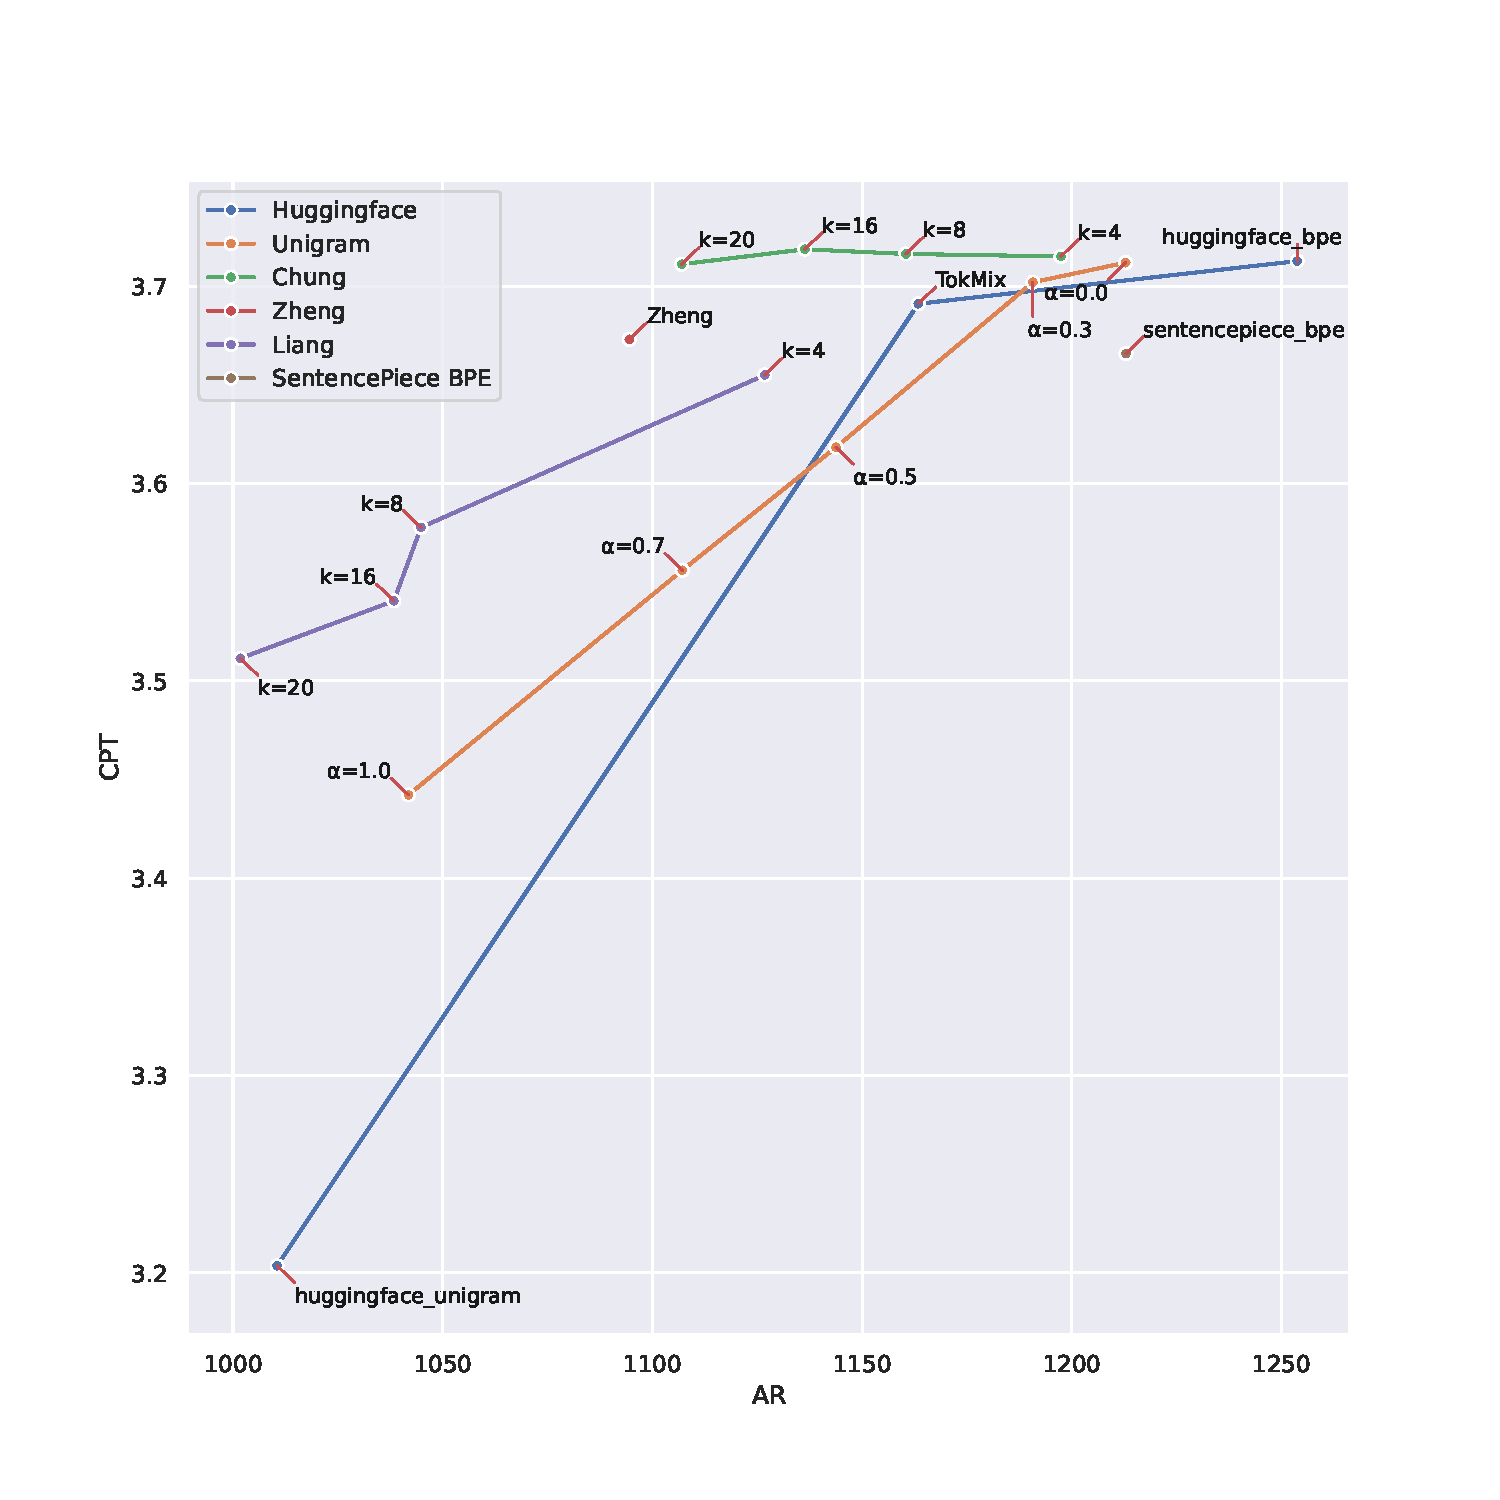
\includegraphics[width=\textwidth]{figures/all_tokenizers_AR_vs_CPT.pdf}
    \caption{We visualize the overall vocabulary allocation metrics for all tokenizers from Table \ref{tab:all_tokenizers_metrics}. We observe that the vocabulary allocation scores are related --- higher AR usually means higher CPT.  We also observe that Huggingface Unigram is a clear outlier, although a combination of separate, monolingual Huggingface Unigrams (TokMix) approaches the performance of the Sentencepiece Unigram with the corresponding data imbalance ($\alpha=0.3$). We see that the balancing methods overperform the unbalanced Unigrams ($\alpha=1.0$, $\alpha=0.7$) in terms of CPT but perform similarly or worse to the simple case of running the Sentencepiece Unigram trainer on a balanced set $\alpha=0.0$.}
    \label{fig:all_tokenizers_AR_vs_CPT}
\end{figure}

Crucially, we see that the reproduced methods of \citet{chung_improving_2020,zheng_allocating_2021,liang_xlm-v_2023} do improve over the unbalanced baselines $\alpha=1.0, 0.7, 0.5$ on the CPT metric, especially with a higher number of clusters but do not outperform the simple case of training the Sentencepiece Unigram on a balanced dataset $\alpha=0.0$. We also observe that the clustering methods with a higher number of clusters along with Zheng are close to each other on the CPT-AR plot. We assume this is because, with higher $k$, the clustering methods reduce to the Zheng method (training separate tokenizers for each language). Similarly, with a lower number of clusters, the methods are much closer to the vanilla Sentencepiece Unigram trained on an unbalanced dataset.

\begin{figure}
    \centering
    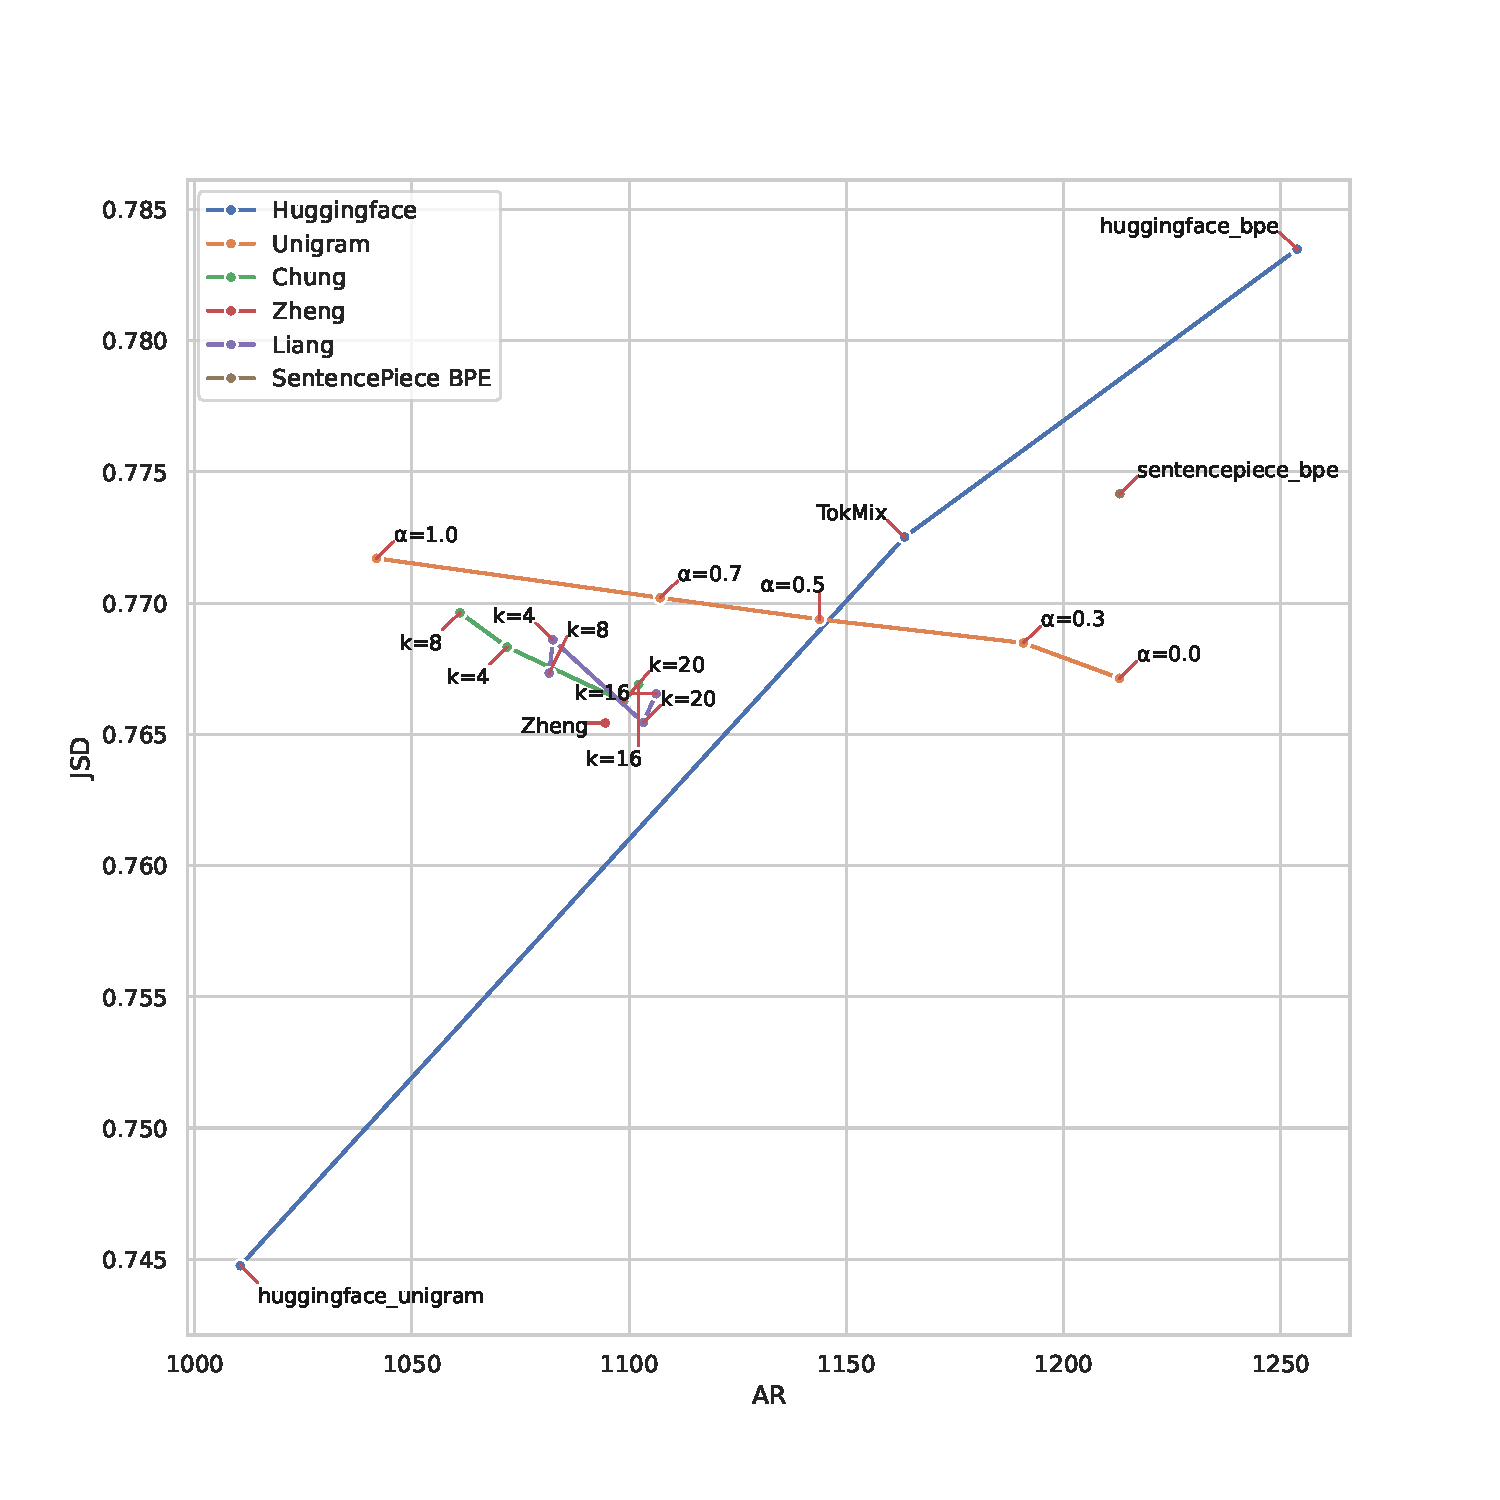
\includegraphics[width=\textwidth]{figures/all_tokenizers_AR_vs_JSD.pdf}
    \caption{We visualize the tokenizers from Table \ref{tab:all_tokenizers_metrics} in terms of Average Rank and Jensen-Shannon Divergence. Here we can see that all methods based on Sentencepiece result in similar overlap independent of the allocation. This is interesting because the replicated balancing methods (Chung, Zheng, Liang) work by splitting the data and training separate tokenizers. Nevertheless, after merging the separate subtokenizers they all seem to end up with similar vocabulary overlaps. The highest vocabulary isolation is surprisingly achieved by the Huggingface BPE tokenizer, which is contrary to the hypothesis stated by \citet{chung_improving_2020,zheng_allocating_2021} that the tokenizers trained on the concatenation of all data tend to select subwords shared across all languages.}
    \label{fig:all_tokenizers_AR_vs_JSD}
\end{figure}

We also explore the relationship between vocabulary allocation and vocabulary overlap on the \autoref{fig:all_tokenizers_AR_vs_JSD}\footnote{The CPT-JSD plot is similar but is less readable therefore we present the relationship between AR and JSD}. We see that the differences between all methods based on Sentencepiece are small compared to the differences between Huggingface tokenizers. This is surprising because one of the motivations for the method of Chung and Liang is to promote overlap between similar languages while minimizing the overlap between distant languages. We would therefore expect the overall overlap to decrease, as the number of spurious token sharing decreases. Nevertheless, we observe that the resulting overlap is lower or similar to our Sentencepiece Unigram tokenizers. Similarly, the Zheng method works by training separate tokenizers for each language and then combining them into one. We would expect the overlap to be even lower than the original Sentencepiece Unigram but we observe that the overlap is comparable. 
Surprisingly, the lowest vocabulary overlap (highest JSD) is achieved by the Huggingface BPE trained on a combined corpus. 

\begin{figure}
    \centering
    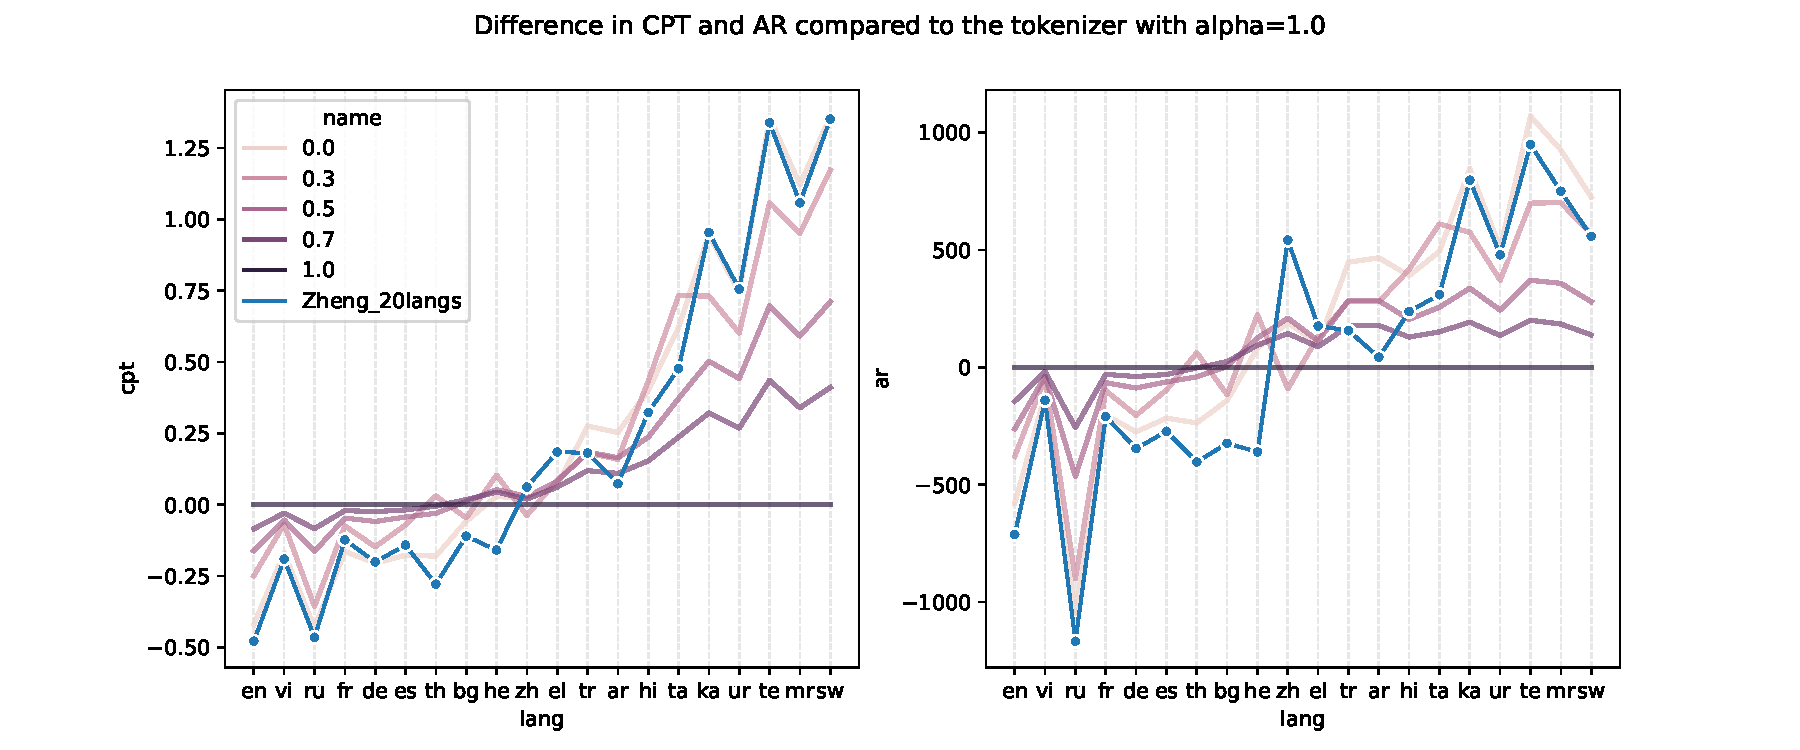
\includegraphics[width=\textwidth]{figures/zheng_vs_alphas.pdf}
    \caption{We zoom into the results of the Zheng method and compare the vocabulary allocation across the individual languages represented by this tokenizer against the backdrop of the vanilla Unigram tokenizers trained with different data imbalances from \ref{fig:data_balance_vs_allocation_per_lang}. We observe a striking similarity between the vocabulary allocation of the Zheng tokenizer and the Unigram tokenizer with $\alpha=0.0$, especially in terms of characters per token. This comes as a large surprise because the Zheng method works by training a separate tokenizer for each language and then merging them. Despite the different methods of obtaining the vocabulary, the resulting tokenizers are very similar across the languages.}
    \label{fig:zheng_vs_alphas}
\end{figure}

We investigate the differences between the balanced Unigram and the replicated methods in more detail by examining the CPT and AR metrics computed \textbf{per language}. We use the data balance experiments from \autoref{sec:tokenizer_training_with_data_imbalance} for comparison. We start by comparing the Zheng method with the increasingly imbalanced Unigram tokenizers in \autoref{fig:zheng_vs_alphas}. We plot the increase or decrease in vocabulary allocation metrics for each language sorted by the data available. Remarkably, we see that the Zheng method is strikingly similar in terms of CPT and AR per language to the Unigram tokenizer trained on the balanced set $\alpha=0.0$. The similarity seems to be higher in the CPT metric although the AR metric is also very similar, especially for the highest and lowest resource languages. We find this result quite surprising because of the distinctness of the Zheng method --- it trains a separate tokenizer for each language and then merges the vocabularies together. Nevertheless, the resulting tokenizers are very similar to the Unigram tokenizer trained on the balanced set. This result seems to validate the choice of the ALP metric for the selection of vocabulary sizes in the Zheng method (see \autoref{fig:zheng_vs_alphas_alp}) but it also calls into question the necessity of the separate training of tokenizers for each language. One advantage of the Zheng method is that splitting the data into separate languages lowers the memory requirements for the training of the separate Sentencepiece Unigram. However, this comes at a cost of higher overall compute time because of the need for training hundreds of tokenizers to be able to select the ones that maximize the overall ALP after merging them.


\begin{figure}[H]
    \centering
    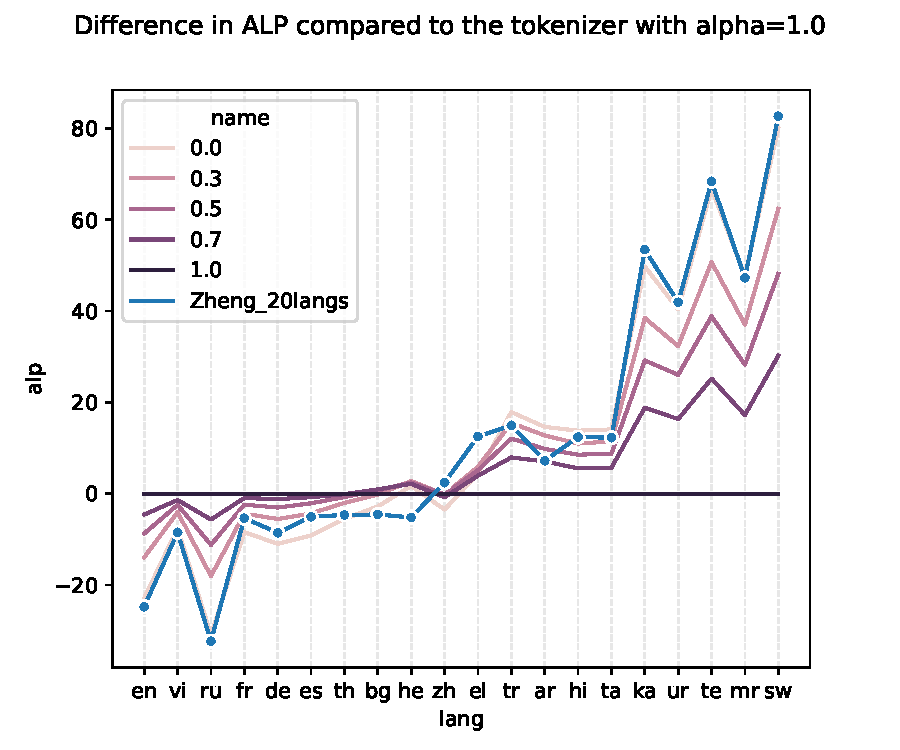
\includegraphics[width=0.7\textwidth]{figures/zheng_vs_alphas_alp.pdf}
    \caption{Intrigued by the similarity between the Zheng tokenizer and the Unigram tokenizer with $\alpha=0.0$ from Figure \ref{fig:zheng_vs_alphas} we also look at the ALP metric which is used for the selection of vocabulary sizes in the Zheng method. Here we see that the greedy optimization of ALP across languages indeed results in a similar vocabulary allocation as the Unigram tokenizer with $\alpha=0.0$.}
    \label{fig:zheng_vs_alphas_alp}
\end{figure}

\begin{figure}[H]
    \centering
    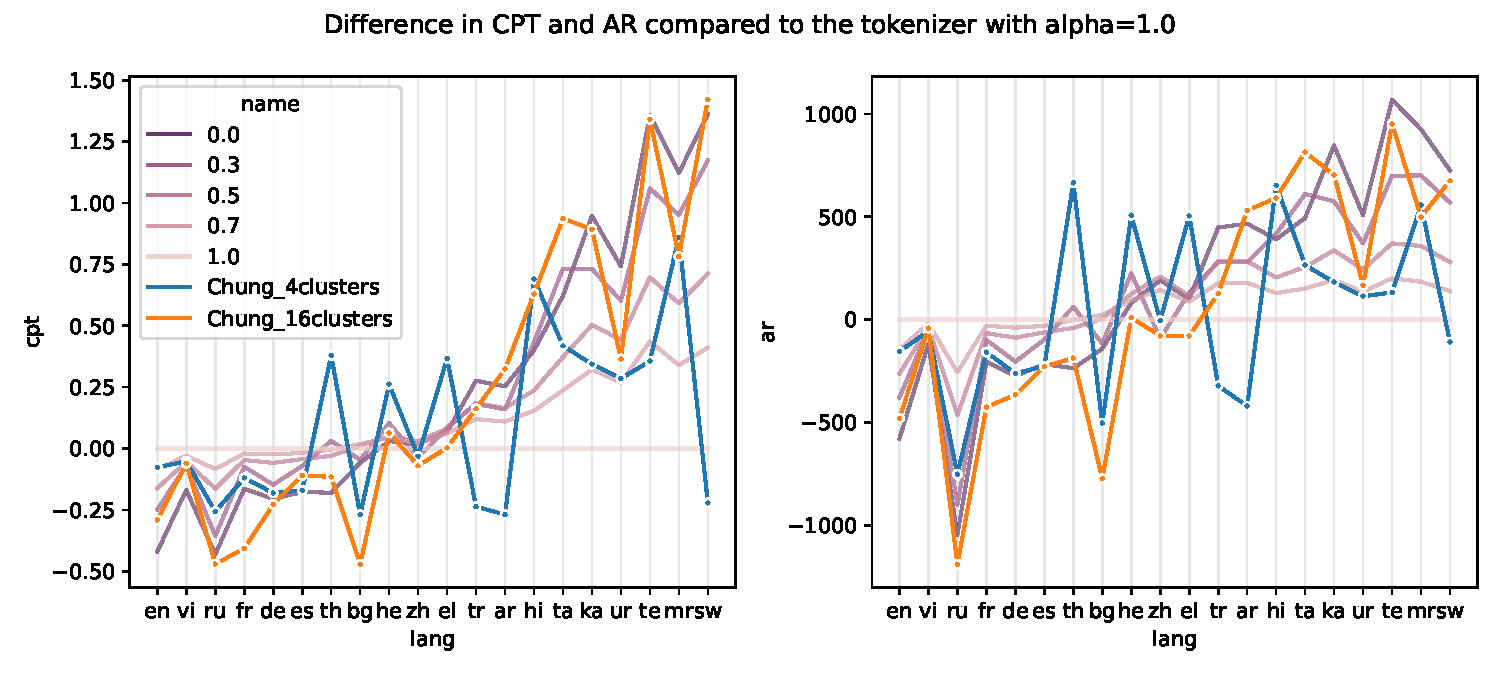
\includegraphics[width=\textwidth]{figures/chung_vs_alphas.pdf}
    \caption{Here we inspect the language-level vocabulary allocation of the Chung method. Similarly to the Zheng method, the Chung method also performs similarly to the Unigram tokenizer with $\alpha=0.0$. Unfortunately, we believe this is an artifact of the choice of our training data for the Chung method. We use a balanced dataset ($\alpha=0.0$) for training the cluster-specific tokenizers. The balance of the data seems to be more important than the clustering step. After merging the cluster-specific tokenizers, the resulting tokenizer is very similar to the Unigram tokenizer with $\alpha=0.0$.}
    \label{fig:chung_vs_alphas}
\end{figure}

Next, we inspect the Chung method and compare it in detail to our Unigram tokenizers in \autoref{fig:chung_vs_alphas}. For comparison, we select a run with a low number of clusters (k=4) and a high number of clusters (k=16). We see that the different numbers of clusters yield different results. In the case of a higher number of clusters, we see that the tokenizer exhibits a similar trend in CPT and AR across the languages as the balanced Unigram tokenizer with $\alpha=0.0$ albeit with some deviations. In the case of a lower number of clusters, the metrics per language seem to be more distinct compared to our Unigram tokenizers. 

We look at the CPT per language for k=16 more closely and identify the languages where the Chung tokenizer differs significantly from the Unigram tokenizer with $\alpha=0.0$. We see that the CPT drops significantly for Bulgarian (bg), Urdu (ur), Marathi (mr), and to some degree French (fr). On the other hand, we see smaller improvements for English (en), Vietnamese (vi), Spanish (es), Thai (th), Hindi (hi), and Tamil (ta). We compare this to the cluster assignments in \autoref{tab:chung_clusters_k16}. Revealingly, we observe that all languages with the large drop in CPT have been assigned to a cluster with another, higher-resource language. Bulgarian is assigned with Russian (8th largest corpus versus 3rd largest corpus), Urdu with Arabic (17th vs. 13th), Marathi with Hindu (18th vs. 14th) and French with English (4th vs. 1st)

We continue with a similar analysis for the 4 clusters. We see that the CPT for Bulgarian (bg), Turkish (tr), Arabic (ar), and Swahili (sw) is lower than any of our Unigram tokenizers. On the other hand, we see significant improvements for Thai (th), Hebrew (he), Greek (el), and Hindi (hi) over our Unigram tokenizers. Additionally, Marathi (mr) achieves the highest CPT increase over the unbalanced Unigram baseline, although the increase stays in the range of the $\alpha=0.5$ Unigram tokenizer. We again look at the cluster assignments in \autoref{tab:chung_clusters_k4}. We observe that Bulgarian and Arabic are assigned to a cluster with higher-resource Russian (3rd) and Chinese, which could explain the decrease in CPT for the two. Similarly, Swahili and Turkish which use the Latin script are assigned to a cluster with higher resource English (largest corpus) and Vietnamese (2nd largest). On the other hand, we see that Thai, Hebrew, and Greek are assigned to a cluster with lower-resource languages --- Tamil (ta), Georgian (ka), Urdu (ur), and Telugu (te). As we have observed, Thai, Hebrew, and Greek benefit from this assignment while the lower-resource languages seem to have a lower CPT than the $\alpha=0.7$ Unigram and therefore approach the unbalanced baseline.

\begin{figure}[H]
    \centering
    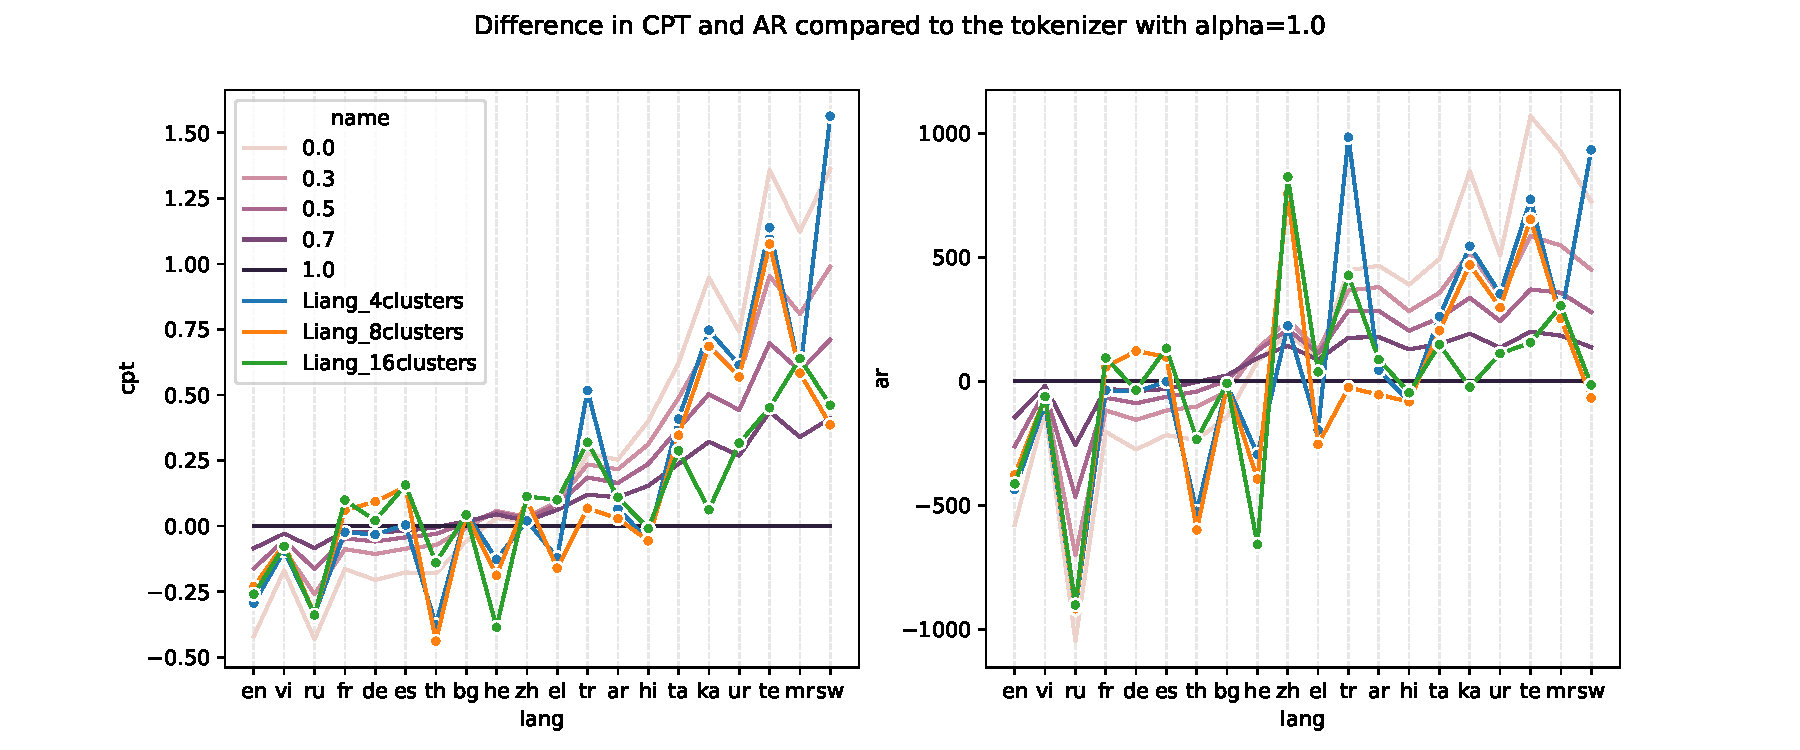
\includegraphics[width=\textwidth]{figures/liang_vs_alphas.pdf}
    \caption{We inspect the language-level vocabulary allocation of the Liang method. We see similarities to the Chung method in \autoref{fig:chung_vs_alphas}. The main differences seem to be the improved Chinese and Arabic for 4 clusters and worse Hebrew and better Urdu for 16 clusters. Overall the results are similar.}
    \label{fig:liang_vs_alphas}
\end{figure}

We look at the \citet{liang_xlm-v_2023} replication results in \autoref{fig:liang_vs_alphas}. We see that despite a slightly different clustering method and per-cluster vocabulary size selection, the Liang method exhibits similar patterns we observed in the Chung method.

Overall, we infer that the Chung and Liang methods are sensitive to cluster assignments. Because the training data are merged per cluster, if a low-resource language gets assigned to a cluster with a high-resource language, the language imbalance acts in favor of the high-resource language. Bearing this in mind, we know from our experiments in \autoref{sec:tokenizer_training_with_data_imbalance} presented previously, that the benefit of adding more data to the high-resource language is lower than the cost that incurs on the low-resource language. We believe this is the cause of the lower overall CPT and AR for the clustering methods.


\section{Comparison of balancing methods on downstream tasks}

To validate our previous assessment from \autoref{sec:comparison_balancing_methods}, we select two replicated methods by \citet{chung_improving_2020,zheng_allocating_2021}. For the clustering method, we select a low- and high- number of clusters $k=4\text{ and }16$. We compare these replicated tokenization methods to the standard Unigram tokenizers trained on differently balanced datasets with $\alpha=1.0, 0.3\text{ and }0.0$

For each of the six tokenizers, we pretrain a masked language model and probe it on three tasks - natural language inference (NLI), part of speech tagging (POS), and named entity recognition (NER). We run the probe training with three different seeds on each language and report the average results\footnote{Note that even though the probe training is done with three different random seeds, the model pretraining was done only once. The variance between pretraining runs is therefore not measured and the error bars should be interpreted as such.}. We note that the models differ only in the tokenizer used. The architecture and training data are fixed across the pretraining and finetuning runs.


\begin{figure}
    \centering
    \begin{subfigure}{.5\textwidth}
      \centering
      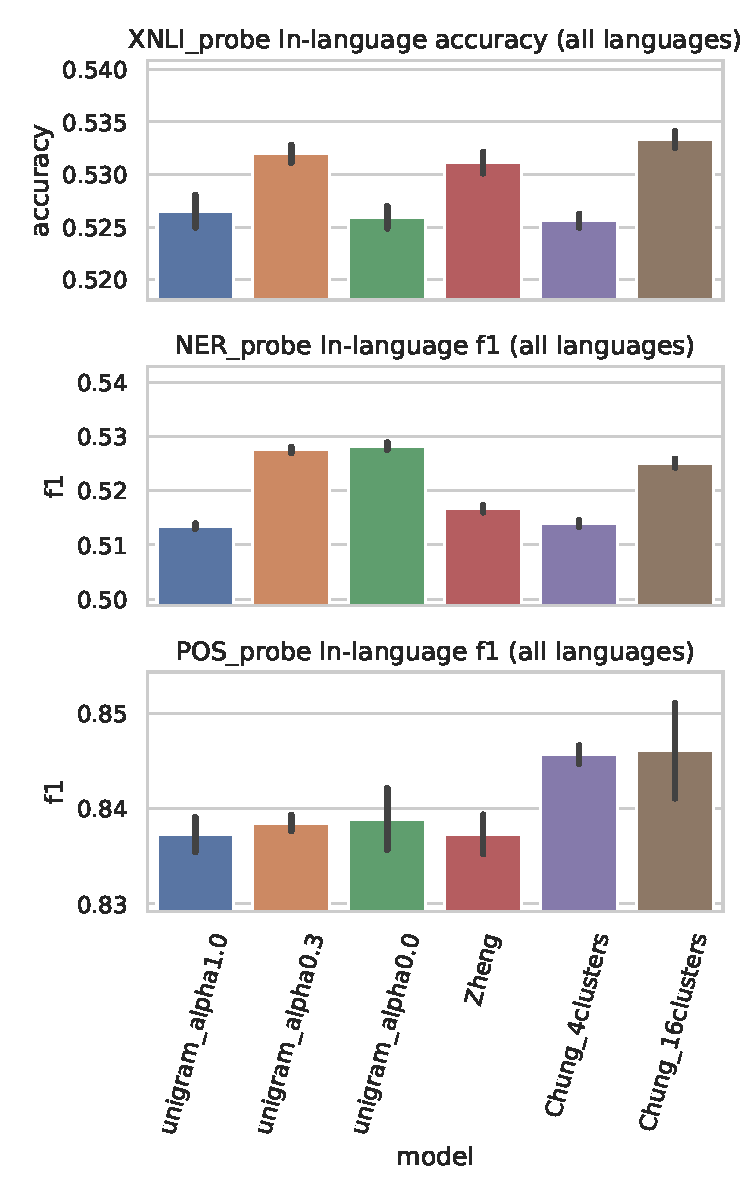
\includegraphics[width=\linewidth]{figures/probe_overall_inlanguage.pdf}
      \caption{In-language results}
      \label{fig:probe_overall_inlanguage}
    \end{subfigure}%
    \begin{subfigure}{.5\textwidth}
      \centering
      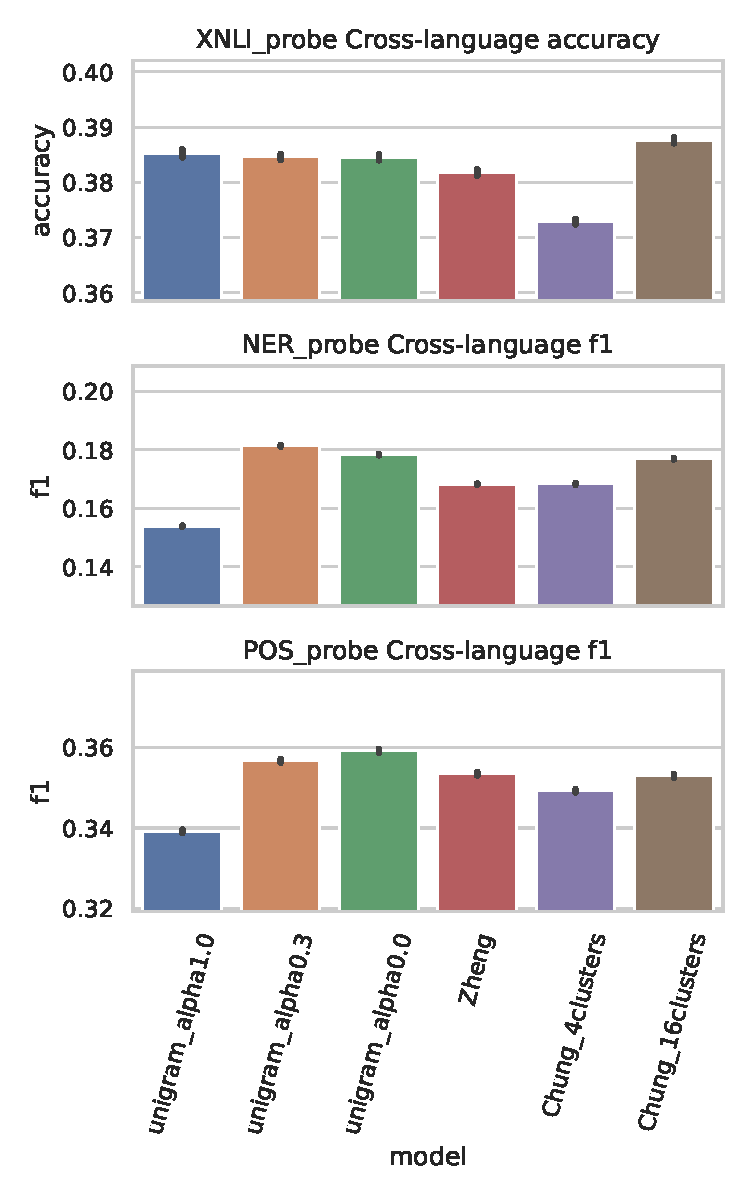
\includegraphics[width=\linewidth]{figures/probe_overall_crosslanguage.pdf}
      \caption{Cross-language results}
      \label{fig:probe_overall_crosslanguage}
    \end{subfigure}
    \caption{We select the replicated methods by \citet{chung_improving_2020,zheng_allocating_2021} and compare them with the vanilla Unigram tokenizers. For comparison, we choose the unbalanced Unigram tokenizer with $\alpha=1.0$ and then two stronger baselines with $\alpha=0.0$ and $\alpha=0.3$ trained on more balanced data. We then pretrain masked language models that differ only in the tokenizer they use and assess the performance of these models on the downstream tasks using probing. We test two settings --- in-language performance, where the model is trained on each of the available languages and then evaluated on the same language, and cross-language performance, where the model is also trained on each language but evaluated on all \textit{but} the training language. The results are a macro average over all the languages (in-language results) or all language pairs (cross-language results). For each model, language, and task we do 3 probe training runs with different random seeds. The error bars represent one standard deviation computed with bootstrapping by randomly sampling seeds for each language.}
    \label{fig:probe_overall}
\end{figure}

In \autoref{fig:probe_overall}, we report the overall in-language and cross-language results for the models. We observe the clearest regularity in cross-language performance for word-level tasks (NER and POS), where all balancing methods improve over the unbalanced $\alpha=1.0$ model. Next, we see higher POS in-language scores for the Chung methods and higher NER in-language scores for the balanced unigrams ($\alpha=0.0\text{ and }0.3$). For in-language NLI, we do not see any systematic effect --- the differences between the models are small ($<1$ percentage point) and the outlier behavior of $\alpha=0.3$ compared to $\alpha=1.0\text{ and }0.0$ suggests that the variance is caused by the finetuning rather than any tokenizer effect.

We inspect the results more closely on the language level. We again compare the performance of the more balanced models to the unbalanced model by plotting the difference in accuracy and F1 score for the tasks by language. The languages are sorted in descending order based on the amount of available data. 



\begin{figure}[H]
    \centering
    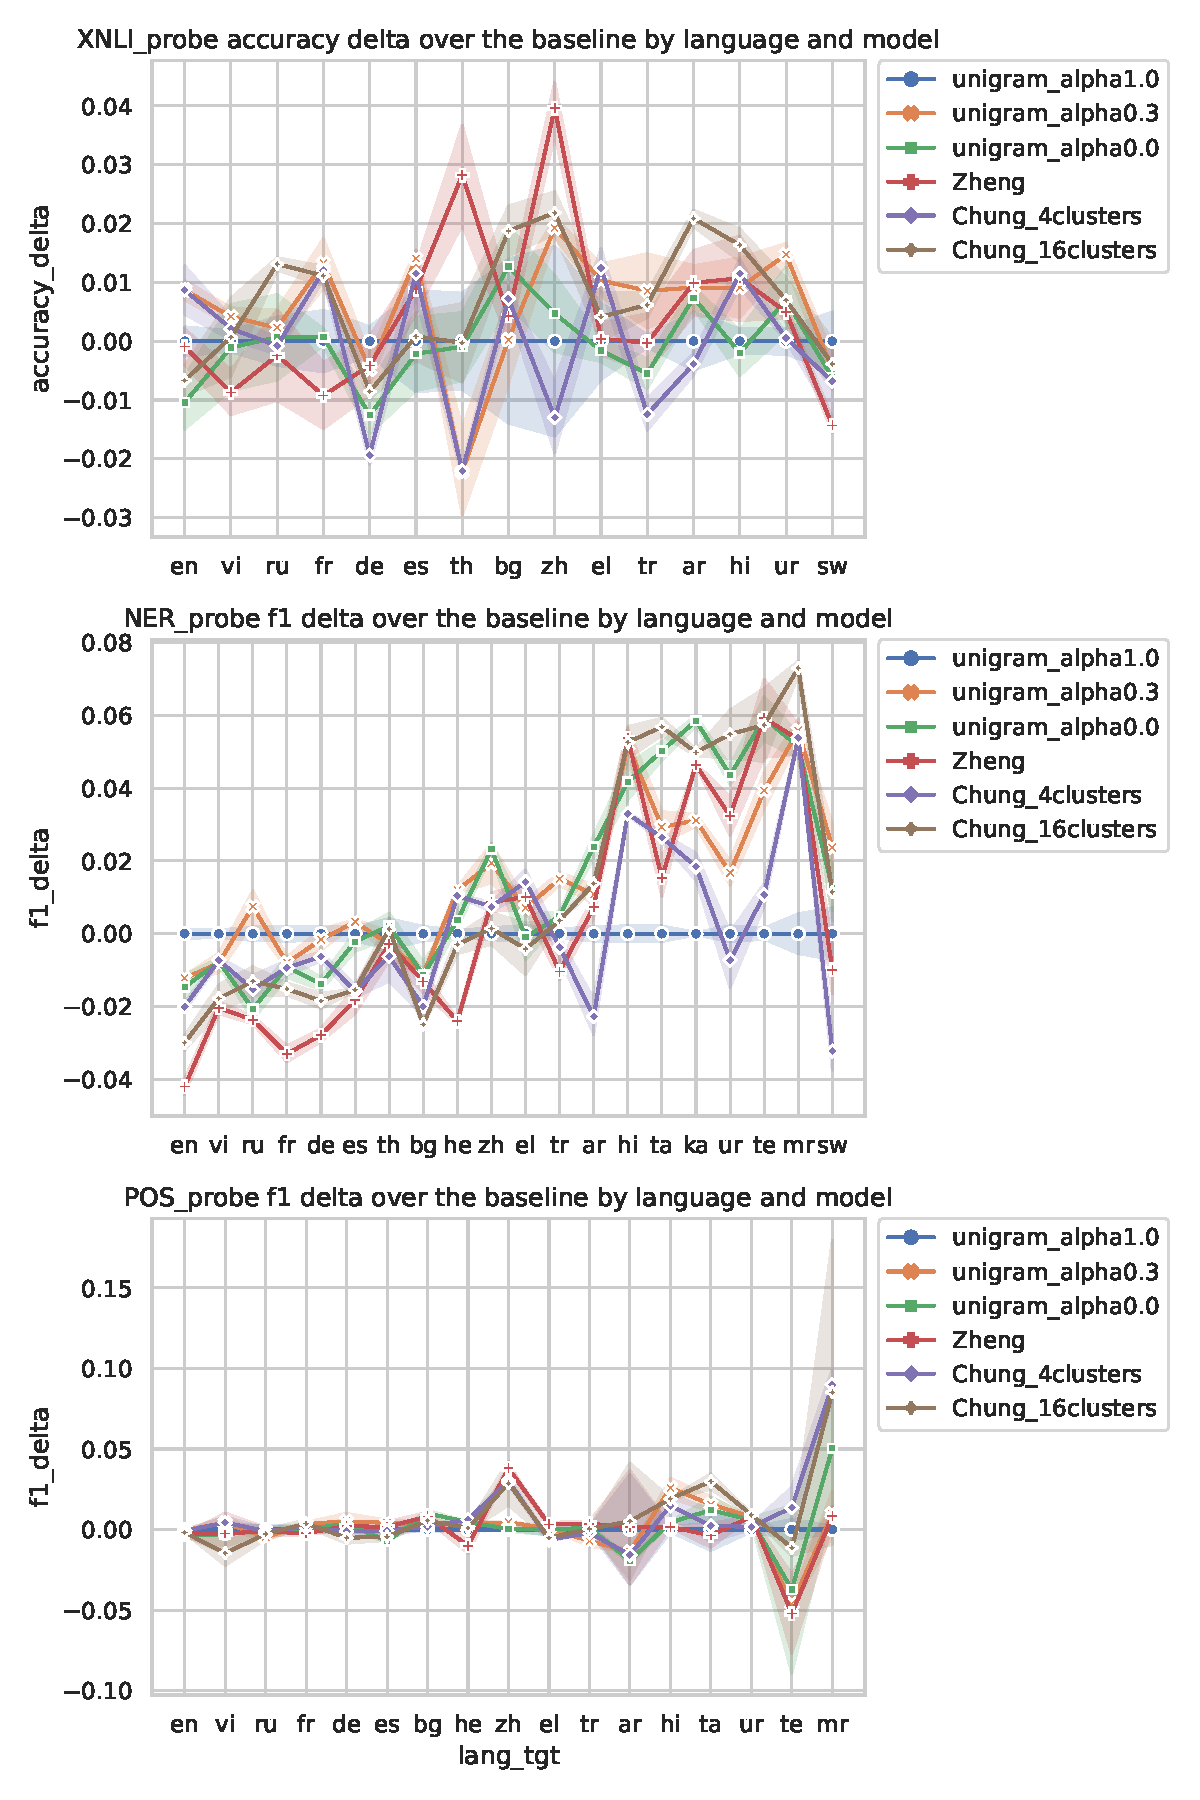
\includegraphics[width=0.8\textwidth]{figures/probe_detailed_inlanguage_over_baseline.pdf}
    \caption{We zoom in on the in-language results from Figure \ref{fig:probe_overall_inlanguage} and compare the performance of the balanced tokenizers against the unbalanced Unigram tokenizer with $\alpha=1.0$ over all tested languages for the tasks. In the case of the word-level tasks, especially in the case of named entity recognition, we observe a clear trend in line with our tokenizer investigations in \ref{fig:chung_vs_alphas}. The balancing methods improve the language representations for word-level tasks. For the sentence-level tasks, we do not observe any systematic effects. This might be in part because the NLI task does not include 4 of our low-resource languages. The error bands are one standard deviation computed from the three probe training runs with different random seeds.}
    \label{fig:probe_overall_inlanguage_over_baseline}
\end{figure}

In \autoref{fig:probe_overall_inlanguage_over_baseline}, we see the in-language results laid out by language. We see a large effect of the probe training language on the NER F1 score and to some degree an effect on the POS F1. We do not see a systematic effect on NLI. For NER, we see the effect of the tokenizer language balance reminiscent of the results in \autoref{fig:zheng_vs_alphas} and \autoref{fig:chung_vs_alphas}. For high-resource languages, we observe a decrease in performance across the board. This is counterbalanced by a larger increase in performance for the low-resource languages. The effect seems to be largest for the $\alpha=0.0$ Unigram tokenizer,ě Zheng method and Chung with 16 clusters. For $\alpha=0.3$ Unigram and Chung with 4 clusters, we see a similar effect but with a smaller magnitude, which is in line with our observations in \autoref{fig:chung_vs_alphas}. In the case of POS, we do see more variance in results towards the low-resource languages but the effect is not as clear as for NER. We see significant improvements with Zheng and Chung methods on Chinese which correspond to the AR improvement for Chinese for the Zheng method in \autoref{fig:zheng_vs_alphas} but we do not see any difference in Chinese tokenizer metrics in the case of Chung (\autoref{fig:chung_vs_alphas}). We also see some improvements in Hindi, Tamil, and Marathi. For Telugu, we see a surprising drop for all methods except Chung with 4 clusters. Note that the variance in the results is larger for the low-resource languages because of smaller test sets.


\begin{figure}[H]
    \centering
    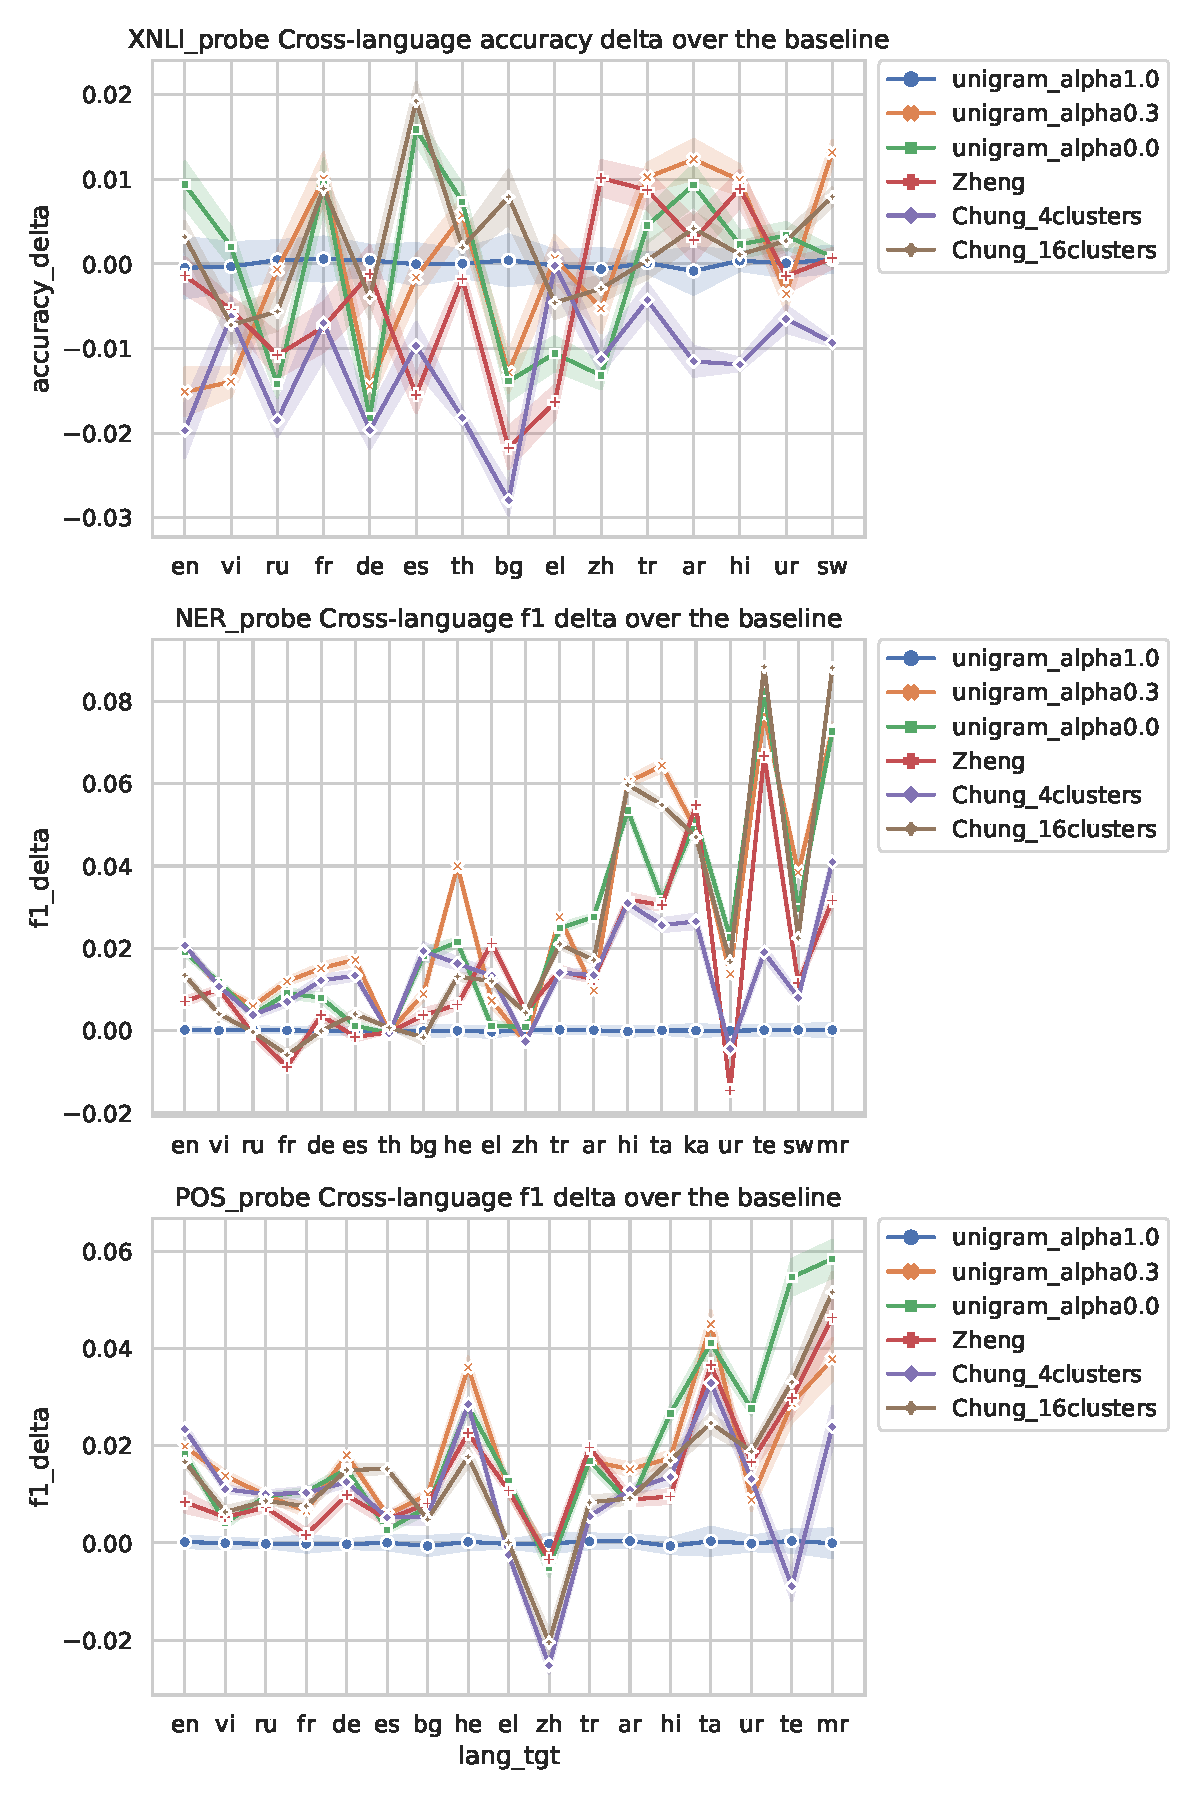
\includegraphics[width=0.8\textwidth]{figures/probe_detailed_crosslanguage_over_baseline_lang_tgt.pdf}
    \caption{Here we investigate in detail the cross-lingual results from Figure \ref{fig:probe_overall_crosslanguage} with comparison to the unbalanced Unigram tokenizer with $\alpha=1.0$. We observe that word-level task transfers behave in line with the tokenizer investigations in \ref{fig:chung_vs_alphas}. Moreover, it seems that both high-resource and low-resource languages benefit from the balancing methods, although the change is most clear on the low-resource side. For the sentence-level tasks, we do not observe any systematic effects. The value for each language and model is computed by averaging the difference in cross-lingual performance for the given \textit{target} language over the baseline. In other words for a given language L we compute the mean performance over all probe trainings done on languages other than L and then evaluate them on language L.}
    \label{fig:probe_overall_crosslanguage_over_baseline}
\end{figure}

We turn our attention to the cross-language results in \autoref{fig:probe_overall_crosslanguage_over_baseline}. Here we again do not see any patterns in the NLI task, other than an overall drop in performance for Chung with 4 clusters, for which we do not have an explanation. On the other hand, we see clear patterns in NER and POS tasks. For both tasks, we see that the performance for low-resource languages is improved over the unbalanced baseline. Moreover, we see that the balancing has a net positive effect even for the high-resource languages, although the effect is not as pronounced as for the low-resource languages. In the NER task, we see that the Chung method with 4 clusters does not seem to improve on low-resource language as much as the other methods. 

Lastly, we plot the differences in tokenizer metrics against the differences in downstream task scores in scatter matrices. In \autoref{fig:probe_overall_inlanguage_scattermatrix} we show the in-language results and in \autoref{fig:probe_overall_crosslanguage_scattermatrix} we show the cross-language results. In the case of in-language results, we see that for the NER and POS tasks, there is a significant Spearman correlation between the differences in tokenizer metrics and the differences in task performance (0.84 and 0.34 Spearman correlation respectively). For the NLI task, we do not observe any significant correlations. This is in line with our observations from the language-level results (\autoref{fig:probe_overall_inlanguage_over_baseline}). In the case of cross-language results, we observe significant, low, negative Spearman correlations between JSD and word-level tasks NER and POS (-0.21 and -0.22 respectively). We also see significant correlations between CPT/AR and all downstream tasks (0.14 for NLI, 0.39 for NER, and 0.29 for POS)\footnote{Because for cross-lingual transfer we test pairs of languages, we compute the combined CPT for the pair of languages as an average between the CPT of the source and target languages.}.

Collecting all our observations together, we see that the tokenizers that aim to balance low-resource and high-resource languages do influence the results of downstream tasks compared to an unbalanced tokenizer. We see that the effect varies by task and language. Generally, we see a high influence on word-level tasks (NER and POS) and no significant influence on NLI. In the case of in-language results, the effect of increasing the vocabulary allocation for low-resource languages and decreasing allocation for high-resource languages is clear for the NER task (\autoref{fig:probe_overall_inlanguage_over_baseline}). In the case of cross-lingual transfer, this effect is clear on both word-level tasks and, interestingly, is a net positive even for the high-resource tasks (\autoref{fig:probe_overall_crosslanguage_over_baseline}). For all cases where the balancing effect is clear (NER in-language, NER/POS cross-language), the best overall performance is achieved by the Unigram tokenizer trained on a balanced train set with $\alpha=0.0\text{ and }0.3$ (\autoref{fig:probe_overall}). For in-language POS, we see the best performance for the Chung method. To quantify the strength of the influence of tokenizer improvement on task improvement, we plot the metrics and downstream results in a scatterplot matrix and compute Spearman correlations between them. For all cases where the balancing effect is clear, we see significant correlations between the differences in tokenizer metrics and the differences in downstream task performance (\autoref{fig:probe_overall_inlanguage_scattermatrix} and \autoref{fig:probe_overall_crosslanguage_scattermatrix}). In general, the correlations we observe suggest that improving vocabulary allocation (CPT, AR) has a positive effect on in-language and cross-language performance on word-level tasks. Moreover, higher vocabulary overlap (lower JSD) also seems to have a positive effect on word-level tasks, although the effect is smaller. 
% Moreover, we also observe significant correlations between inlanguage POS and CPT/AR and significant, low correlation between crosslanguage NLI and CPT/AR

\begin{figure}[H]
    \centering
    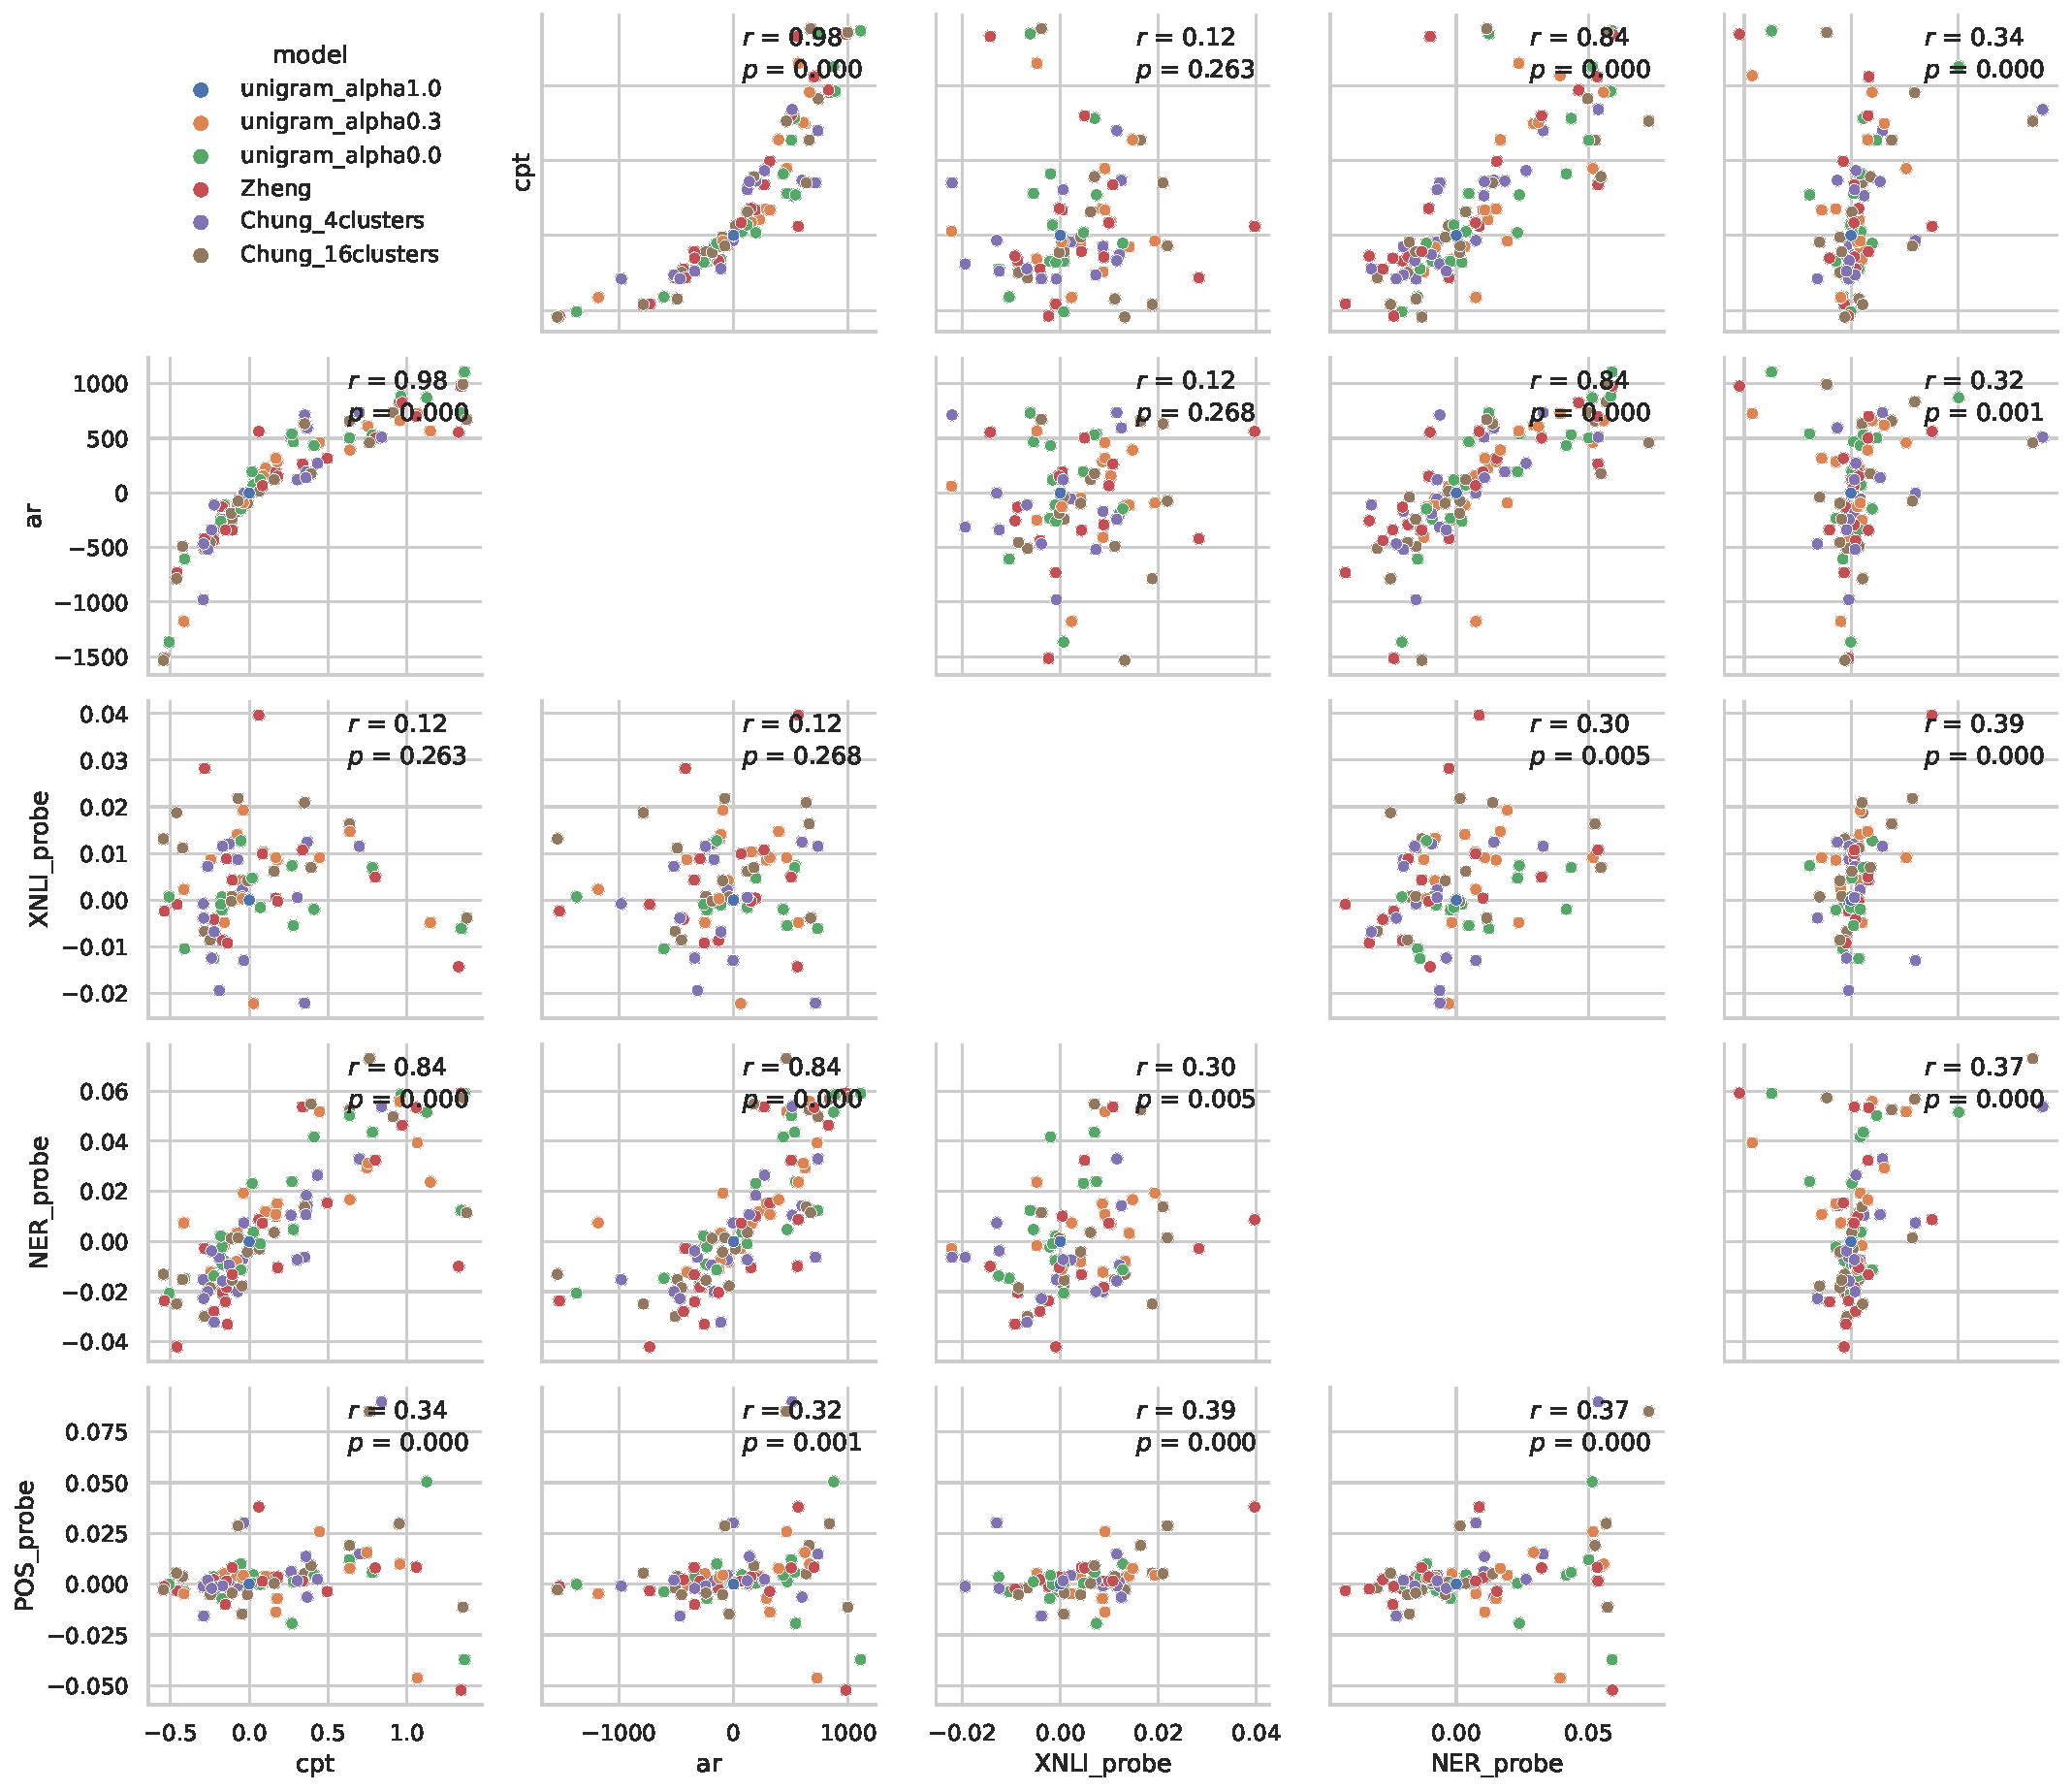
\includegraphics[width=\textwidth]{figures/probe_detailed_inlanguage_scattermatrix.pdf}
    \caption{We visualize the in-language results from Figure \ref{fig:probe_overall_inlanguage} in a scatter matrix. We \tomaszrep{center the results for each language and then plot the differences from the mean performance against the differences in our tokenizer metrics}{substract mean result across three tokenization mwethods from per-language results}. We see significant Spearman correlations for the NER and POS tasks, although for POS the correlation is low. For the NLI task, we do not observe any significant correlations.}
    \label{fig:probe_overall_inlanguage_scattermatrix}
\end{figure}

\begin{figure}[H]
    \centering
    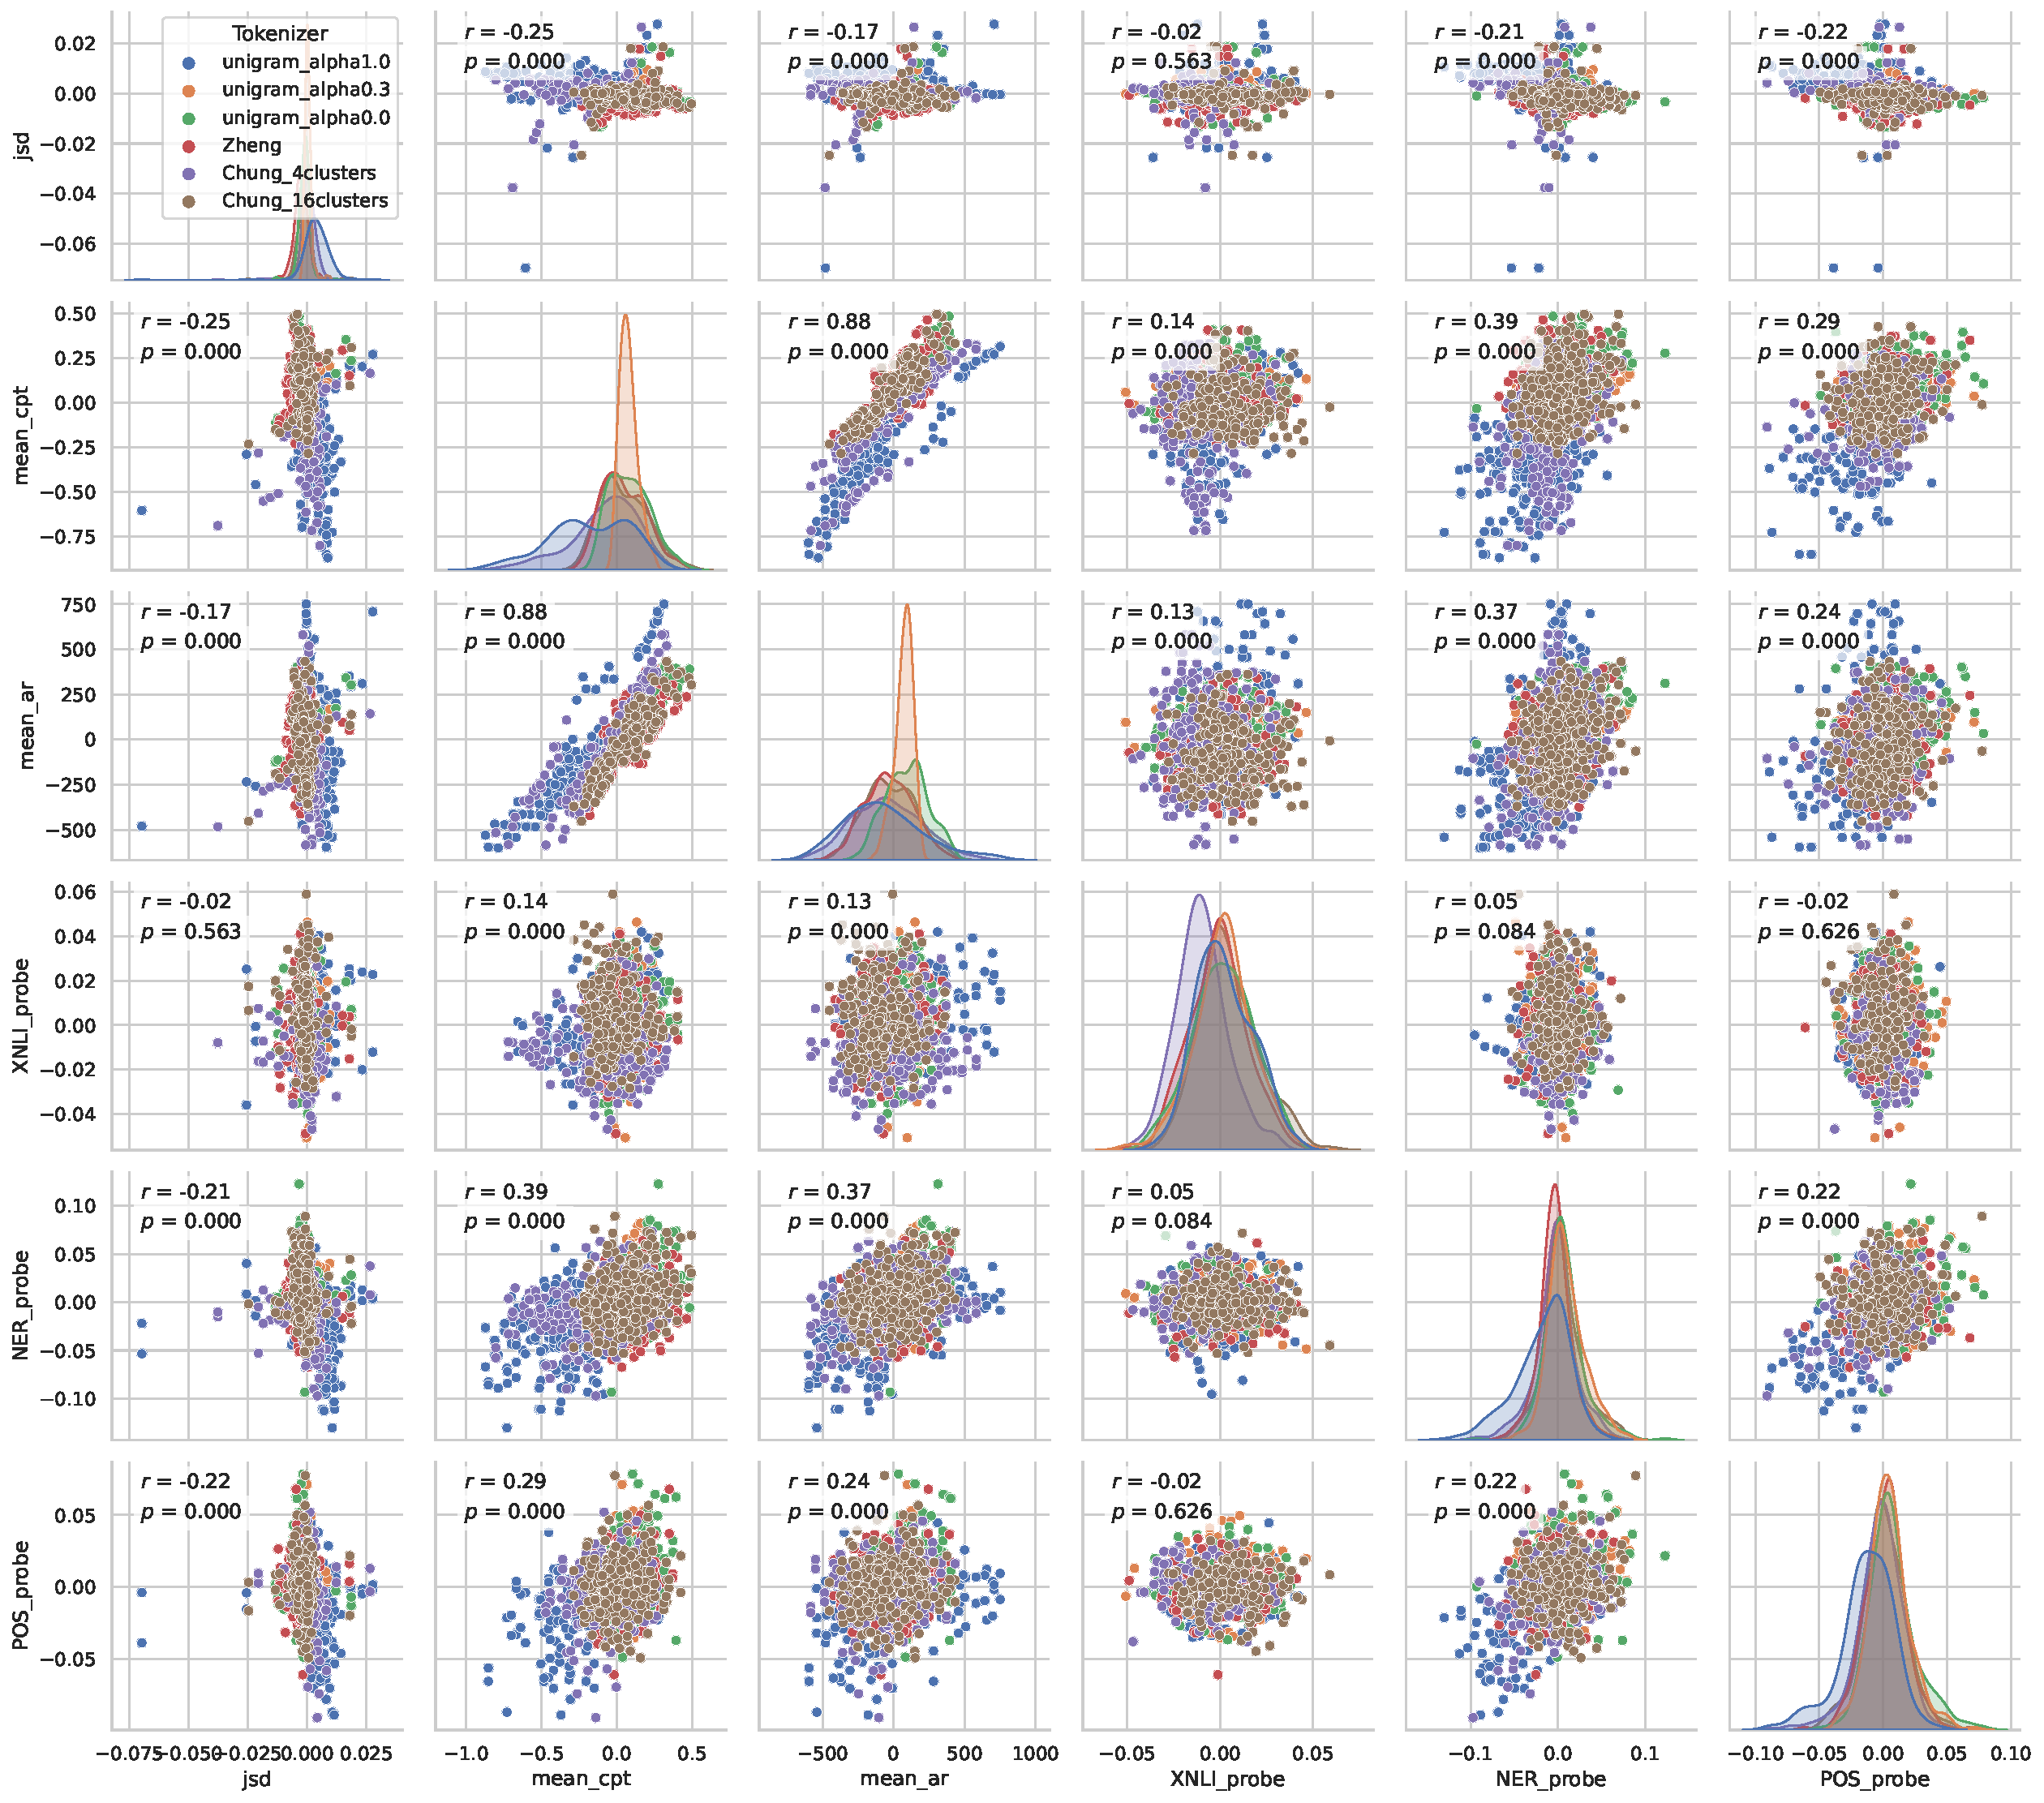
\includegraphics[width=\textwidth]{figures/probe_detailed_crosslanguage_scattermatrix.pdf}
    \caption{We visualize the cross-language results from Figure \ref{fig:probe_overall_crosslanguage} in a scatter matrix. We \tomaszrep{center the results for each language and then plot the differences from the}{substract mean performance across the three models from the language pairs results} of vocabulary overlap metric (JSD) and the combined CPT/AR of the source and target languages. We see significant, very low negative correlations between JSD and F1 scores for the NER and POS tasks and higher, significant correlations between combined CPT and F1 scores. This suggests that the word-level tasks benefit only very slightly from an increase in overlap (decrease in JSD) and an increase in token length in source and target languages. For the NLI task, we observe a significant, low correlation between combined CPT/AR and NLI accuracy. This suggests that the cross-lingual transfer for sentence-level tasks benefits from an increase in token length in source and target languages.}
    \label{fig:probe_overall_crosslanguage_scattermatrix}
\end{figure}
